\documentclass[12pt]{article}

\usepackage{fixltx2e}
\usepackage{textcomp}
\usepackage[cm]{fullpage}
\usepackage{amsfonts}
\usepackage{verbatim}
\usepackage[english]{babel}
\usepackage{pifont}
\usepackage{color}
\usepackage{setspace}
\usepackage{lscape}
\usepackage{indentfirst}
\usepackage[normalem]{ulem}
\usepackage{booktabs}
% \usepackage{nag}
\usepackage{natbib}
% \usepackage{bibtex}
\usepackage{float}
\usepackage{latexsym}
\usepackage{hyperref}
\usepackage{url}
% \usepackage{html}
\usepackage{epsfig}
\usepackage{graphicx}
\usepackage{amssymb}
\usepackage{amsmath}
\usepackage{bm}
\usepackage{array}
%\usepackage{mhchem}
\usepackage{ifthen}
\usepackage{caption}
\usepackage{xcolor}
\usepackage{amsthm}
\usepackage{amstext}
\usepackage{nicefrac}
\usepackage{algorithm}
\usepackage{algorithmic}
\usepackage[scientific-notation=true]{siunitx}
\usepackage{subfigure}
\usepackage[flushleft]{threeparttable}
\usepackage{lineno}
\usepackage{adjustbox}
\usepackage{ragged2e}
\usepackage{authblk}
\usepackage{multirow}
\usepackage[T1]{fontenc}

\setlength{\parskip}{1em}
\renewcommand{\baselinestretch}{2.0}
\renewcommand\Affilfont{\small}
\renewcommand{\thefigure}{S\arabic{figure}}
\renewcommand{\thetable}{S\arabic{table}}
\renewcommand{\thealgorithm}{S\arabic{algorithm}}

\newcommand\ontop[2]{\genfrac{}{}{0pt}{}{#1}{#2}}

\begin{document}

\title{Supplementary material for StarBEAST2}
\author[1,2]{Huw A. Ogilvie\thanks{huw.ogilvie@anu.edu.au}}
\author[2,3]{Remco R. Bouckaert}
\author[2,3]{Alexei J. Drummond}
\affil[1]{Division of Evolution, Ecology and Genetics, Research School of Biology, Australian National University, Canberra, Australia}
\affil[2]{Centre for Computational Evolution, University of Auckland, Auckland, New Zealand}
\affil[3]{Department of Computer Science, University of Auckland, Auckland, New Zealand}

\maketitle

\clearpage

\section{Supplementary figures}

\justifying

\begin{figure}[htb!]
\centering
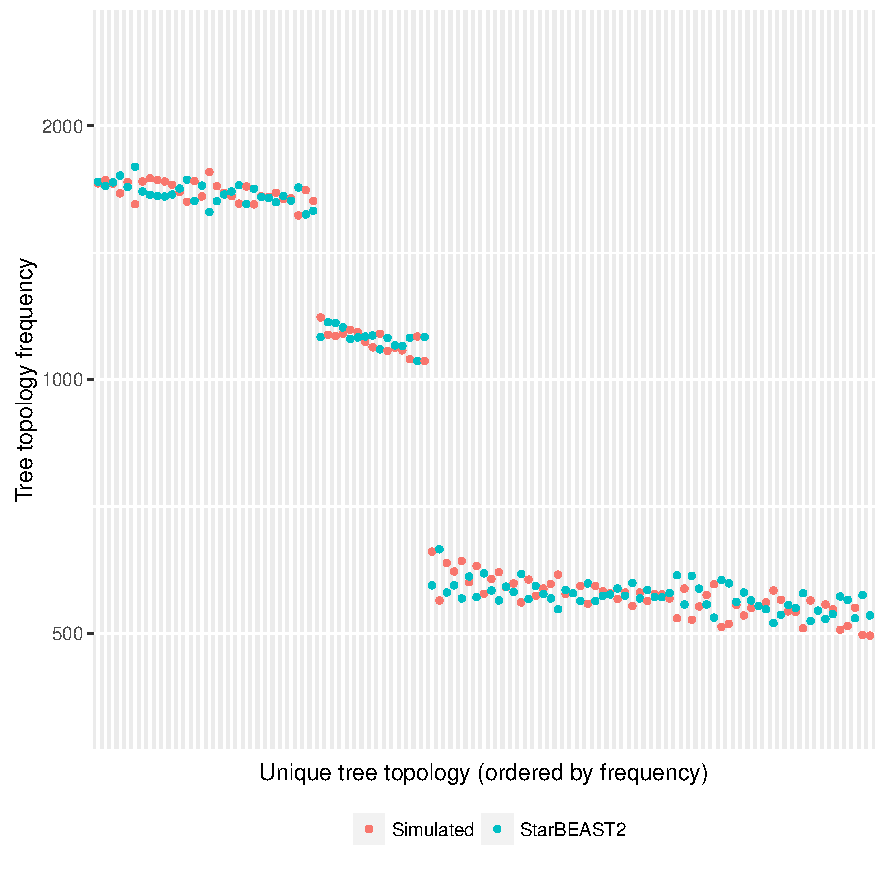
\includegraphics[width=16cm]{species_topology_frequencies.pdf}
\caption
{Frequency of five-taxon species tree topologies sampled from a birth-death prior
distribution. Topologies were sampled by simulating trees using biopy (red), or
by using a StarBEAST2 MCMC chain (blue). Frequencies are identical apart from
noise, indicating that StarBEAST2 is mathematically correct. Three levels of
probability are evident from left to right --- high probability balanced
topologies e.g. ((a,b),((c,d),e)), middle probability intermediate topologies
e.g. (((a,b),(c,d)),e), and low probability unbalanced topologies e.g.
((((a,b),c),d),e).}
\label{fig:speciesTopologyFrequencies}
\end{figure}

\clearpage

\begin{figure}[htb!]
\centering
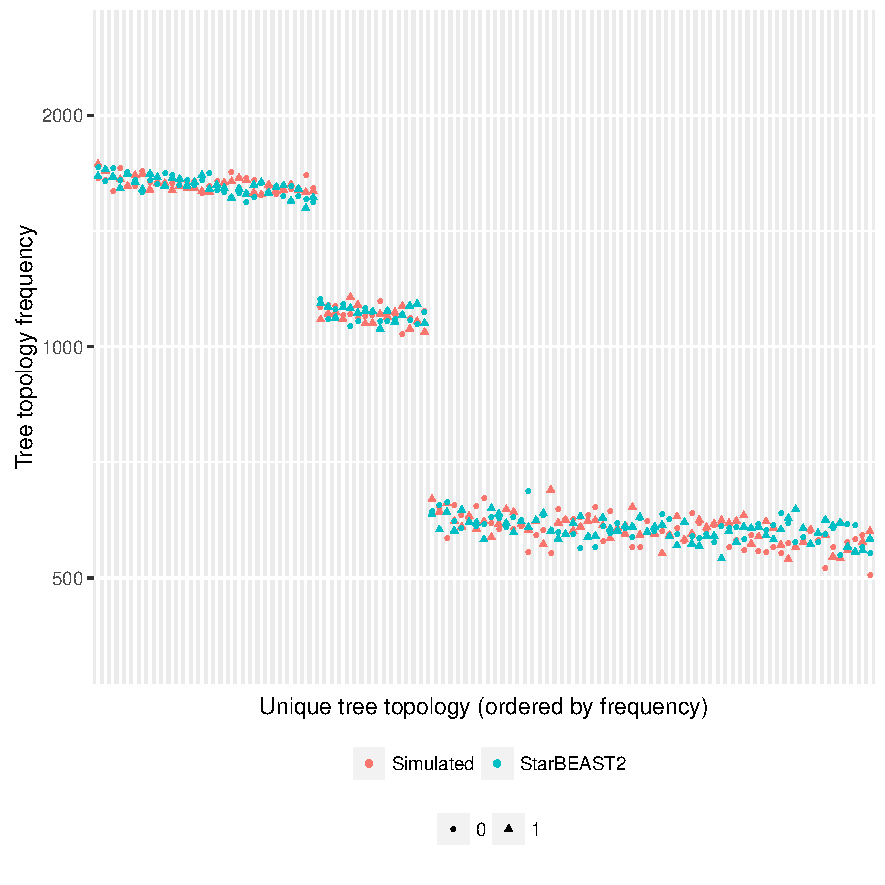
\includegraphics[width=16cm]{gene_topology_frequencies.pdf}
\caption
{Frequency of five-taxon gene tree topologies sampled from a multispecies
coalescent prior distribution. Topologies were sampled by simulating gene trees
within species trees using biopy (red), or by using a StarBEAST2 MCMC chain
(blue). Gene trees were sampled with two clock rates, 0.5 (circles) and 2.0
(triangles), although clock rate should not affect topology or node heights in
units of time. Frequencies are identical apart from noise, indicating that
StarBEAST2 is mathematically correct. Three levels of probability are evident
from left to right --- high probability balanced topologies e.g.
((a,b),((c,d),e)), middle probability intermediate topologies e.g.
(((a,b),(c,d)),e), and low probability unbalanced topologies e.g.
((((a,b),c),d),e).}
\label{fig:geneTopologyFrequencies}
\end{figure}

\clearpage

\begin{figure}[htb!]
\centering
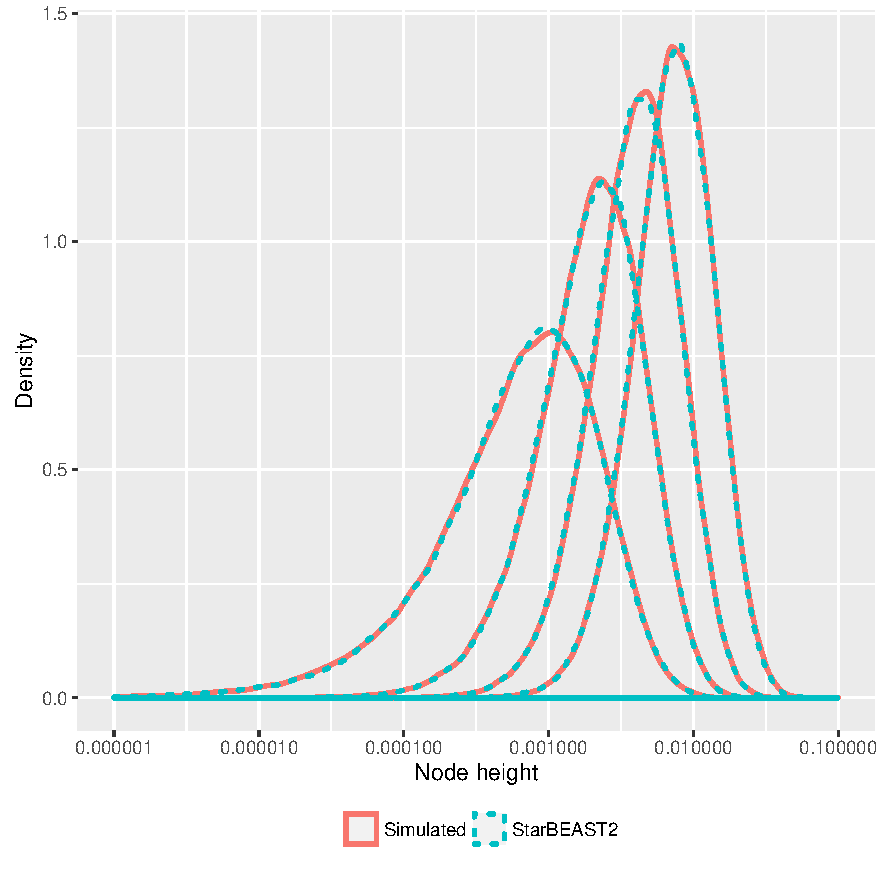
\includegraphics[width=16cm]{species_node_heights.pdf}
\caption
{Probability densities of five-taxon species tree node heights sampled from a
birth-death prior distribution. Node heights were sampled by simulating trees
using biopy (red), or by using a StarBEAST2 MCMC chain (blue). Probability
densities are plotted separately for each ranked node giving four peaks, one
for each internal node. Node height probability densities are identical apart
from noise, indicating that StarBEAST2 is mathematically correct.}
\label{fig:speciesNodeHeights}
\end{figure}

\clearpage

\begin{figure}[htb!]
\centering
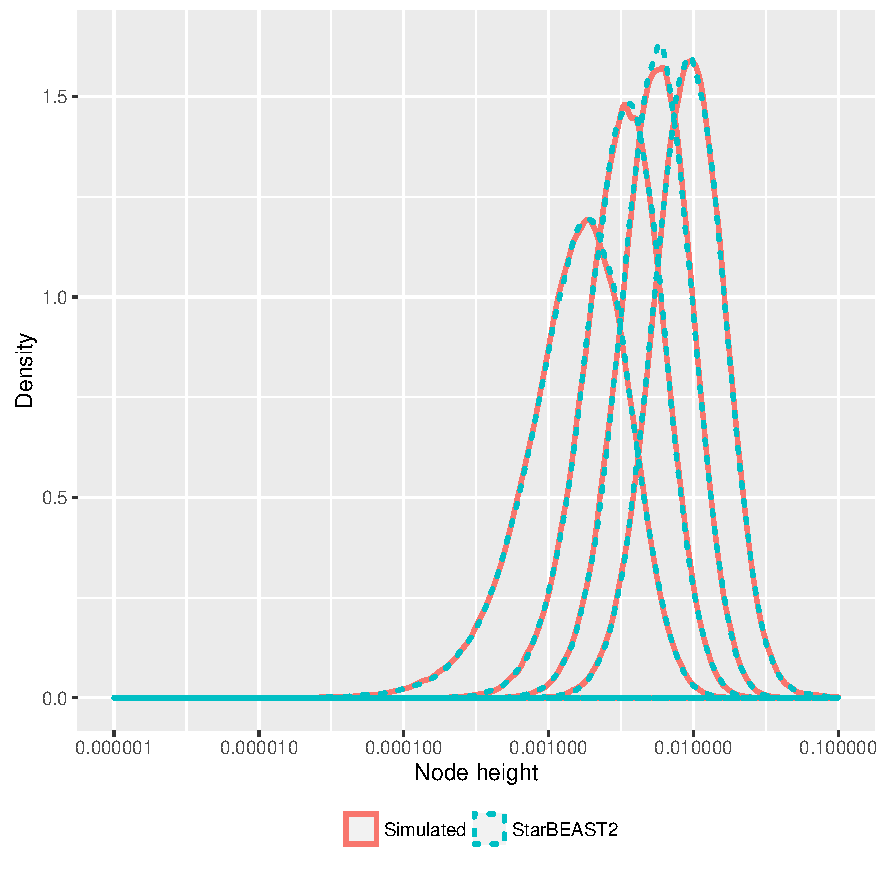
\includegraphics[width=16cm]{gene_node_heights.pdf}
\caption
{Probability densities of five-taxon gene tree node heights sampled from a
multispecies coalescent prior distribution. Node heights were sampled by
simulating gene trees within species trees using biopy (red), or by using a
StarBEAST2 MCMC chain (blue). Gene trees were sampled with two clock rates, 0.5
and 2.0, and node heights from both sets of gene trees were combined as clock
rate should not affect topology or node heights in units of time. Probability
densities are plotted separately for each ranked node giving four peaks, one for
each internal node. Node height probability densities are identical apart from
noise, indicating that StarBEAST2 is mathematically correct.}
\label{fig:geneNodeHeights}
\end{figure}

\clearpage

\begin{figure}[htb!]
\centering
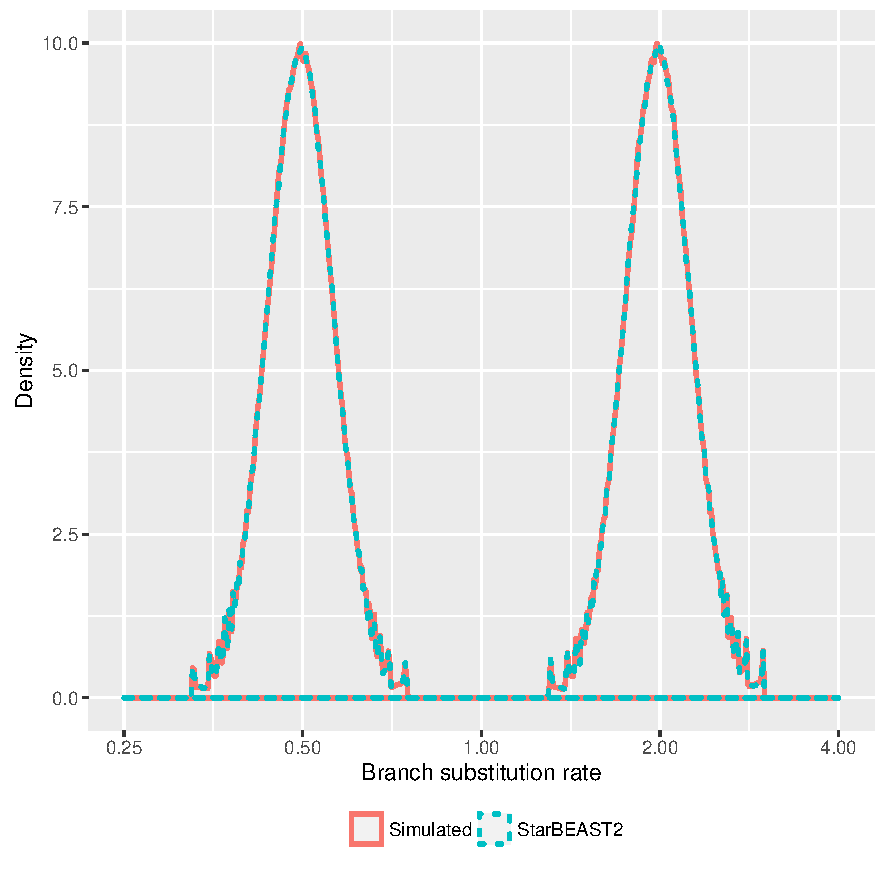
\includegraphics[width=16cm]{gene_branch_rates.pdf}
\caption
{Probability densities of five-taxon gene tree branch rates produced by a
species tree uncorrelated lognormal (UCLN) relaxed clock. Branch rates were
sampled by simulating gene trees within species trees using biopy and simulating
species tree branch rates using scipy (red), or by using a StarBEAST2 MCMC chain
(blue). Gene trees were sampled with two clock rates, 0.5 and 2.0, resulting in
two peaks. Branch rate probability densities are identical apart from noise,
indicating that StarBEAST2 is mathematically correct.}
\label{fig:geneBranchRatesUCLD}
\end{figure}

\clearpage

\begin{figure}[htb!]
\centering
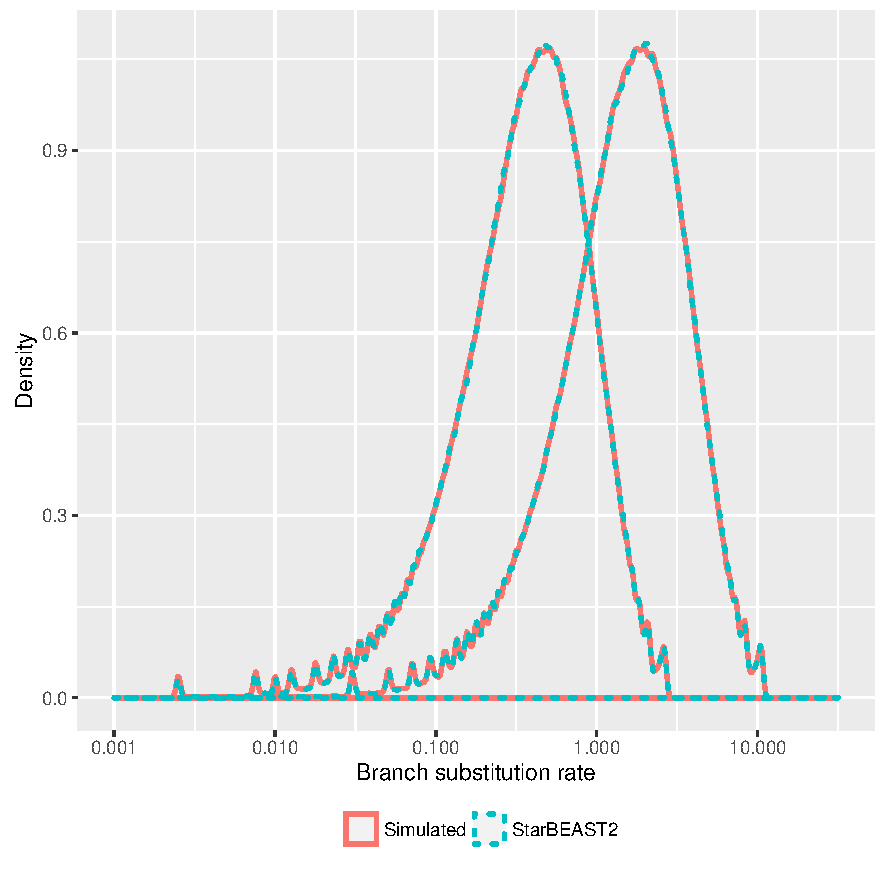
\includegraphics[width=16cm]{exp_gene_branch_rates.pdf}
\caption
{Probability densities of five-taxon gene tree branch rates produced by a
species tree uncorrelated exponential (UCED) relaxed clock. Branch rates were
sampled by simulating gene trees within species trees using biopy and simulating
species tree branch rates using scipy (red), or by using a StarBEAST2 MCMC chain
(blue). Gene trees were sampled with two clock rates, 0.5 and 2.0, resulting in
two peaks. Branch rate probability densities are identical apart from noise,
indicating that StarBEAST2 is mathematically correct.}
\label{fig:geneBranchRatesUCED}
\end{figure}

\clearpage

\begin{figure}[htb!]
\centering
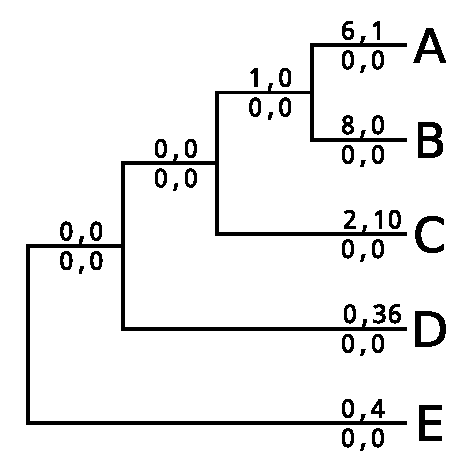
\includegraphics[width=7cm]{false_branch_rates.pdf}
\caption
{Number of erroneous per-species substitution rates estimated using BEAST concatenation and StarBEAST2. Erroneous
branch rates are those with 95\% credibility intervals which do not include the true rate of 1.
Numbers above a branch are the counts of erroneous branches for concatenation, and those
below are the counts for StarBEAST2, both out of 96 replicates. The first count is
the number of branch rates inferred to be faster than 1, and the
second is the number inferred to be slower than 1.}
\label{fig:spilsBranchRates}
\end{figure}

\begin{figure}[htb!]
\centering
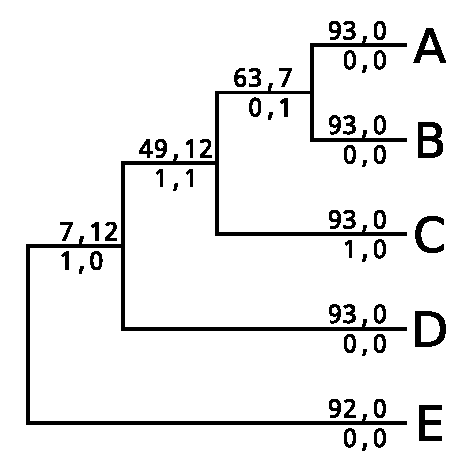
\includegraphics[width=7cm]{false_branch_lengths.pdf}
\caption
{Number of erroneous branch lengths estimated using BEAST concatenation and StarBEAST2. Erroneous
branch lengths are those with 95\% credibility intervals which do not include the true simulated length for a given branch.
Numbers above a branch are the counts of erroneous branches for concatenation, and those
below are the counts for StarBEAST2, both out of 96 replicates. The first count is
the number of branch lengths inferred to be longer than the true length, and the
second is the number inferred to be shorter.}
\label{fig:spilsBranchLengths}
\end{figure}

\clearpage

\begin{figure}[htb!]
\centering
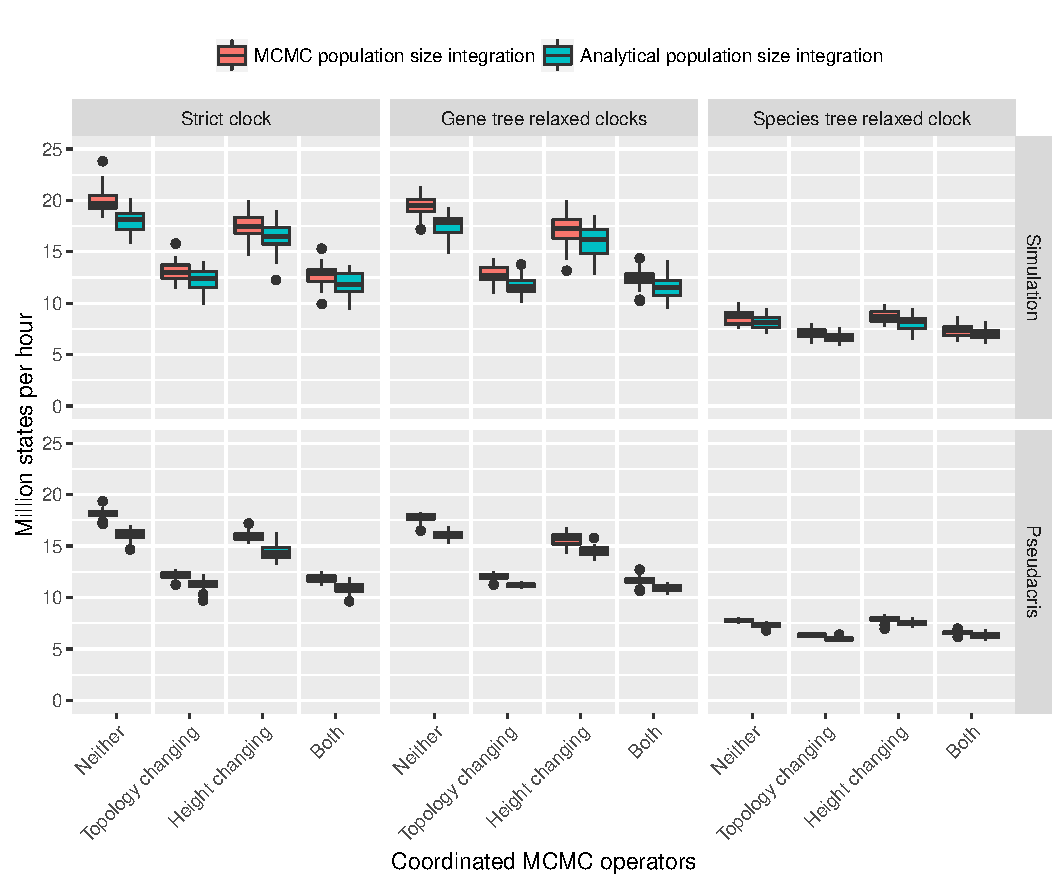
\includegraphics[width=\textwidth]{mstates_per_hour.pdf}
\caption
{Impact of operators, population size integration and clock models on
the calculation time for each state. Topology refers to the
replacement of na\"ive nearest-neighbor interchange and subtree prune and
regraft operators with coordinated operators. Height refers to the addition of
operators which make coordinated changes to node heights. Uncorrelated
log-normal relaxed clocks were applied to either each gene tree (GT-UCLN) or to
the species tree (ST-UCLN). N $\ge$ 30.}
\label{fig:mstatesPerHour}
\end{figure}

\clearpage

% \begin{figure}[htb!]
% \centering
% 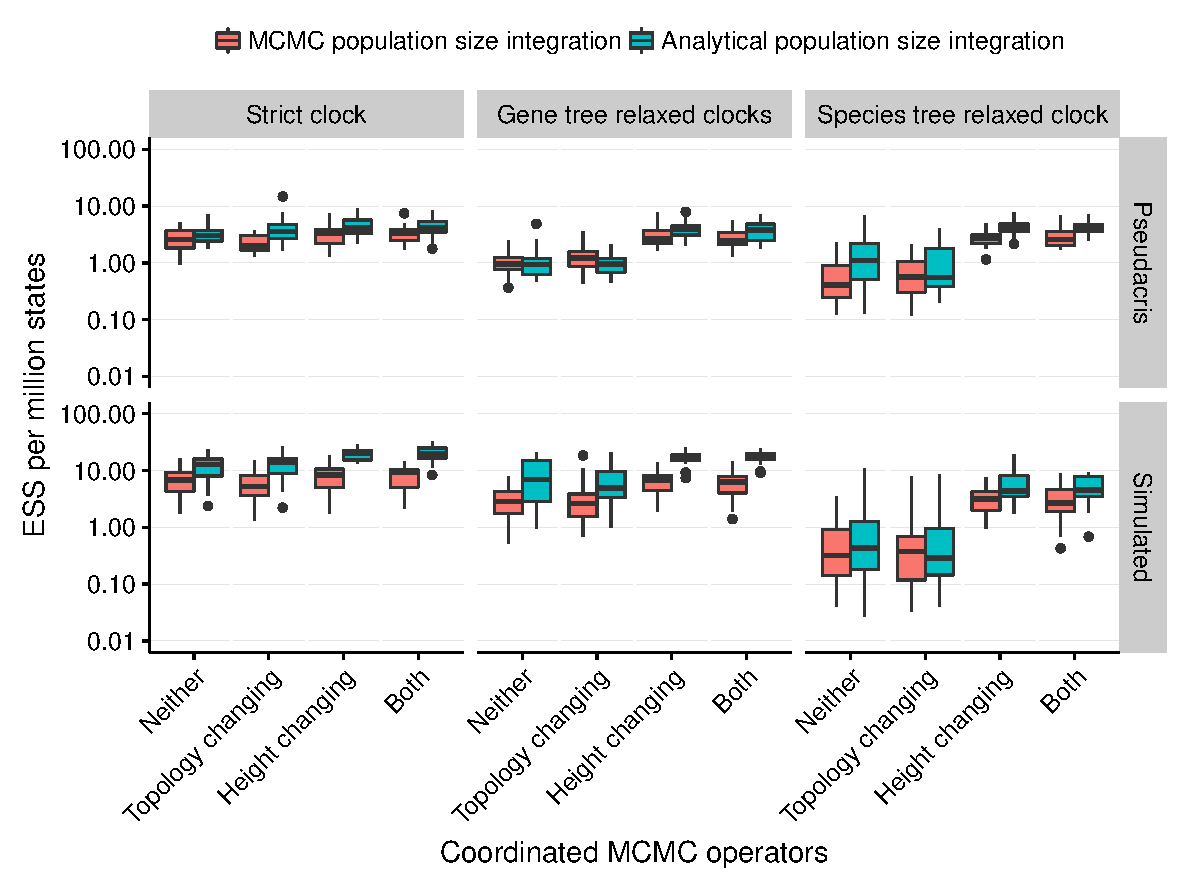
\includegraphics[width=\textwidth]{minimum_ess_per_mstates_starbeast2.pdf}
% \caption
% {Impact of operators, population size integration and clock models on
% estimated sample size (ESS) per million states. Topology refers to the
% replacement of na\"ive nearest-neighbor interchange and subtree prune and
% regraft operators with coordinated operators. Height refers to the addition of
% operators which make coordinated changes to node heights. Uncorrelated log-
% normal relaxed clocks were applied to either each gene tree (GT-UCLN) or to
% the species tree (ST-UCLN). N $\ge$ 22.}
% \label{fig:realEssPerMstates}
% \end{figure}

\clearpage

\begin{figure}[htb!]
\centering
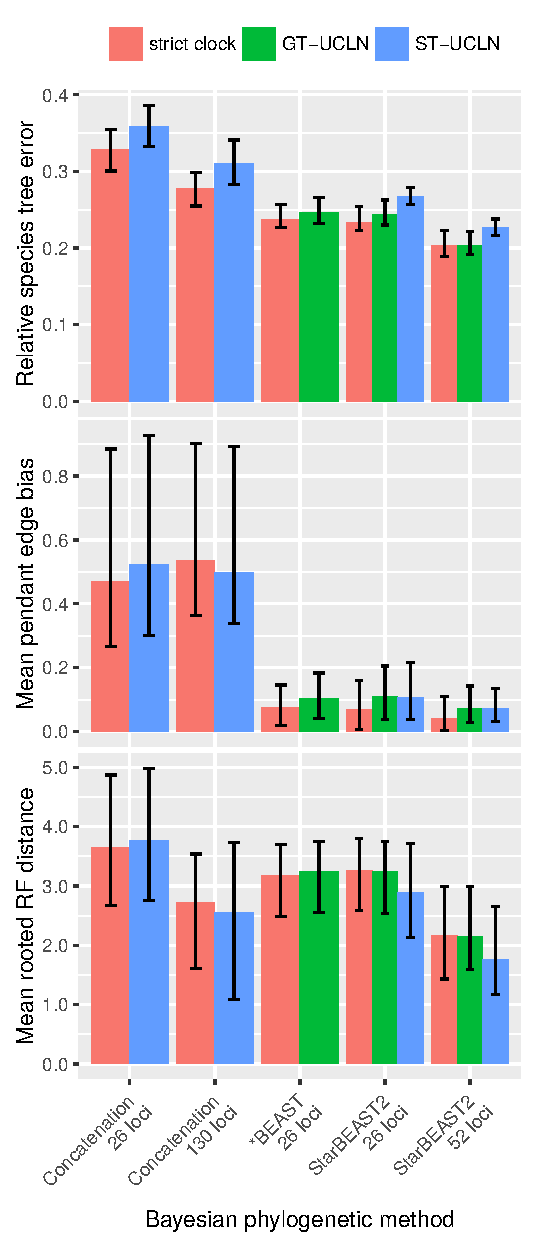
\includegraphics[width=80mm]{tree_error_unphased.pdf}
\caption
{Accuracy of different methods applied to simulated data. Methods are StarBEAST2,
*BEAST and unphased BEAST concatenation with uncorrelated log-normal relaxed clocks applied
to the gene tree (GT-UCLN) or to the species tree (ST-UCLN). (A) Trimmed mean of
relative species tree error, a measure of branch length error. (B) Trimmed
mean of mean pendant edge bias, which measures biased estimates of the ages of
extant species. (C) Trimmed mean of mean rooted Robinson-Foulds (RF) distances, a
measure of topological error. 25\% trim was used to reduce the
influence of outliers. All error bars are 95\% confidence intervals calculated
by bootstrapping. N $\ge$ 22.}
\label{fig:unphasedSpeciesTreeError}
\end{figure}

\clearpage

\begin{figure}[htb!]
\centering
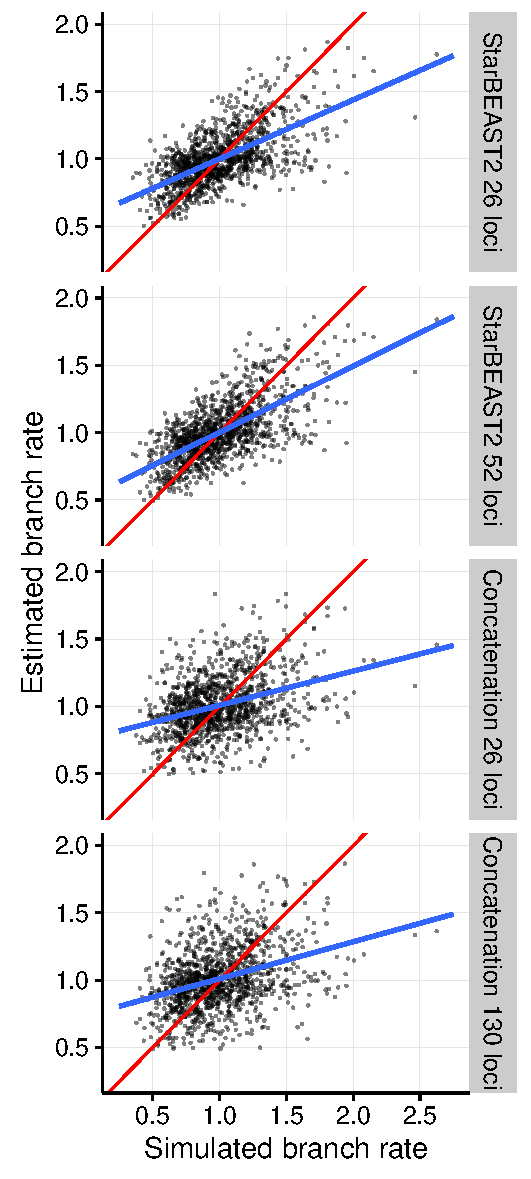
\includegraphics[width=80mm]{branch_rates_unphased.pdf}
\caption
{Estimates of species tree branch rates using unphased BEAST concatenation versus
StarBEAST2. Estimated rates are the posterior expectations of each branch rate
from each replicate. Root branch rates, which were fixed at 1, were excluded.
In blue are simple linear regression lines of best fit, and in red are the $y
= x$ lines showing a perfect relationship between estimates and truth. N $\ge$
22.}
\label{fig:unphasedBranchRates}
\end{figure}

\clearpage

\section{Supplementary tables}

\begin{table}[htb!]
\centering
\caption{Key for tested configurations.}
\label{tab:configurationKey}
\begin{threeparttable}
\begin{adjustbox}{center}
\begin{tabular}{|c|c|c|c|c|c|c|}
\hline
Key & Method & Clock model & Co-ops & Popsizes & Loci & DNA\tabularnewline
\hline
beast-1x-00 & Concatenation & Strict & NA & NA & 26 & Phased\tabularnewline
\hline
beast-1x-01 & Concatenation & Strict & NA & NA & 26 & Unphased\tabularnewline
\hline
beast-1x-20 & Concatenation & ST-UCLN & NA & NA & 26 & Phased\tabularnewline
\hline
beast-1x-21 & Concatenation & ST-UCLN & NA & NA & 26 & Unphased\tabularnewline
\hline
beast-5x-00 & Concatenation & Strict & NA & NA & 130 & Phased\tabularnewline
\hline
beast-5x-01 & Concatenation & Strict & NA & NA & 130 & Unphased\tabularnewline
\hline
beast-5x-20 & Concatenation & ST-UCLN & NA & NA & 130 & Phased\tabularnewline
\hline
beast-5x-21 & Concatenation & ST-UCLN & NA & NA & 130 & Unphased\tabularnewline
\hline
starbeast1-1x-00 & *BEAST & Strict & Neither & MCMC & 26 (50) & Phased\tabularnewline
\hline
starbeast1-1x-10 & *BEAST & GT-UCLN & Neither & MCMC & 26 (50) & Phased\tabularnewline
\hline
starbeast2-1x-00 & StarBEAST2 & Strict & Neither & MCMC & 26 & Phased\tabularnewline
\hline
starbeast2-1x-01 & StarBEAST2 & Strict & Neither & Analytical & 26 & Phased\tabularnewline
\hline
starbeast2-1x-02 & StarBEAST2 & Strict & Heights & MCMC & 26 & Phased\tabularnewline
\hline
starbeast2-1x-03 & StarBEAST2 & Strict & Heights & Analytical & 26 (50) & Phased\tabularnewline
\hline
starbeast2-1x-04 & StarBEAST2 & Strict & Topology & MCMC & 26 & Phased\tabularnewline
\hline
starbeast2-1x-05 & StarBEAST2 & Strict & Topology & Analytical & 26 & Phased\tabularnewline
\hline
starbeast2-1x-06 & StarBEAST2 & Strict & Both & MCMC & 26 & Phased\tabularnewline
\hline
starbeast2-1x-07 & StarBEAST2 & Strict & Both & Analytical & 26 & Phased\tabularnewline
\hline
starbeast2-1x-10 & StarBEAST2 & GT-UCLN & Neither & MCMC & 26 & Phased\tabularnewline
\hline
starbeast2-1x-11 & StarBEAST2 & GT-UCLN & Neither & Analytical & 26 & Phased\tabularnewline
\hline
starbeast2-1x-12 & StarBEAST2 & GT-UCLN & Heights & MCMC & 26 & Phased\tabularnewline
\hline
starbeast2-1x-13 & StarBEAST2 & GT-UCLN & Heights & Analytical & 26 (50) & Phased\tabularnewline
\hline
starbeast2-1x-14 & StarBEAST2 & GT-UCLN & Topology & MCMC & 26 & Phased\tabularnewline
\hline
starbeast2-1x-15 & StarBEAST2 & GT-UCLN & Topology & Analytical & 26 & Phased\tabularnewline
\hline
starbeast2-1x-16 & StarBEAST2 & GT-UCLN & Both & MCMC & 26 & Phased\tabularnewline
\hline
starbeast2-1x-17 & StarBEAST2 & GT-UCLN & Both & Analytical & 26 & Phased\tabularnewline
\hline
starbeast2-1x-20 & StarBEAST2 & ST-UCLN & Neither & MCMC & 26 & Phased\tabularnewline
\hline
starbeast2-1x-21 & StarBEAST2 & ST-UCLN & Neither & Analytical & 26 & Phased\tabularnewline
\hline
starbeast2-1x-22 & StarBEAST2 & ST-UCLN & Heights & MCMC & 26 & Phased\tabularnewline
\hline
starbeast2-1x-23 & StarBEAST2 & ST-UCLN & Heights & Analytical & 26 (50) & Phased\tabularnewline
\hline
starbeast2-1x-24 & StarBEAST2 & ST-UCLN & Topology & MCMC & 26 & Phased\tabularnewline
\hline
starbeast2-1x-25 & StarBEAST2 & ST-UCLN & Topology & Analytical & 26 & Phased\tabularnewline
\hline
starbeast2-1x-26 & StarBEAST2 & ST-UCLN & Both & MCMC & 26 & Phased\tabularnewline
\hline
starbeast2-1x-27 & StarBEAST2 & ST-UCLN & Both & Analytical & 26 & Phased\tabularnewline
\hline
starbeast2-2x-03 & StarBEAST2 & Strict & Heights & Analytical & 52 (100) & Phased\tabularnewline
\hline
starbeast2-2x-13 & StarBEAST2 & GT-UCLN & Heights & Analytical & 52 (100) & Phased\tabularnewline
\hline
starbeast2-2x-23 & StarBEAST2 & ST-UCLN & Heights & Analytical & 52 (100) & Phased\tabularnewline
\hline
\end{tabular}
\end{adjustbox}
\begin{tablenotes}
\item Loci numbers in brackets are for \textit{Crocidura} reanalyses
\end{tablenotes}
\end{threeparttable}
\end{table}

\begin{landscape}

\begin{table}[htb!]
\centering
\caption{Ln(ESS per hour) convergence for simulated data.}
\label{tab:simulatedPerHour}
\begin{threeparttable}
\begin{adjustbox}{center}
\renewcommand{\arraystretch}{1.5}
\tiny
$\begin{array}{|c|c|c|c|c|c|c|c|c|c|c|}
\hline
\text{key} & \text{extinctionfraction} & \text{likelihood} & \text{minimum} & \text{netdiversificationrate} & \text{popmean} & \text{posterior} & \text{prior} & \text{speciescoalescent} & \text{speciestree} & \text{treeheight}\tabularnewline
\hline
\text{beast-1x-00} & 7.598\pm0.135 & 6.129\pm0.184 & 5.865\pm0.197 & 7.904\pm0.125 & NA & 5.967\pm0.182 & 6.085\pm0.390 & NA & 8.183\pm0.137 & 8.214\pm0.128\tabularnewline
\hline
\text{beast-1x-01} & 7.200\pm0.369 & 5.736\pm0.242 & 5.313\pm0.288 & 7.486\pm0.441 & NA & 5.482\pm0.259 & 5.424\pm0.381 & NA & 8.349\pm0.339 & 8.347\pm0.364\tabularnewline
\hline
\text{beast-1x-20} & 7.271\pm0.260 & 5.969\pm0.286 & 5.109\pm0.374 & 7.252\pm0.343 & NA & 5.745\pm0.247 & 5.391\pm0.310 & NA & 6.407\pm0.403 & 5.335\pm0.550\tabularnewline
\hline
\text{beast-1x-21} & 6.689\pm0.325 & 5.717\pm0.171 & 4.890\pm0.358 & 6.691\pm0.368 & NA & 5.457\pm0.186 & 5.044\pm0.268 & NA & 6.181\pm0.417 & 5.116\pm0.491\tabularnewline
\hline
\text{beast-5x-00} & 5.437\pm0.145 & 3.679\pm0.231 & 3.585\pm0.248 & 5.865\pm0.195 & NA & 3.618\pm0.256 & 4.372\pm0.478 & NA & 6.373\pm0.222 & 6.754\pm0.326\tabularnewline
\hline
\text{beast-5x-01} & 4.878\pm0.289 & 3.305\pm0.232 & 3.196\pm0.256 & 5.163\pm0.383 & NA & 3.204\pm0.262 & 3.671\pm0.398 & NA & 6.090\pm0.367 & 6.302\pm0.413\tabularnewline
\hline
\text{beast-5x-20} & 3.503\pm0.782 & 2.976\pm0.521 & 0.333\pm0.868 & 3.051\pm0.644 & NA & 2.894\pm0.475 & 2.981\pm0.517 & NA & 1.216\pm0.549 & 0.333\pm0.868\tabularnewline
\hline
\text{beast-5x-21} & 3.300\pm0.632 & 2.743\pm0.313 & 0.218\pm0.617 & 2.929\pm0.592 & NA & 2.602\pm0.273 & 2.659\pm0.347 & NA & 0.930\pm0.551 & 0.220\pm0.619\tabularnewline
\hline
\text{starbeast1-1x-00} & 6.123\pm0.370 & 4.480\pm0.341 & 3.716\pm0.589 & 6.240\pm0.498 & 5.224\pm0.380 & 4.662\pm0.808 & 4.179\pm0.164 & 4.563\pm0.779 & 6.533\pm0.564 & 4.139\pm0.956\tabularnewline
\hline
\text{starbeast1-1x-10} & 5.063\pm0.532 & 4.339\pm0.319 & 2.043\pm0.447 & 4.135\pm0.392 & 3.040\pm0.275 & 2.368\pm0.290 & 3.542\pm0.312 & 2.345\pm0.287 & 2.526\pm0.300 & 2.059\pm0.451\tabularnewline
\hline
\text{starbeast2-1x-00} & 6.624\pm0.385 & 5.376\pm0.405 & 4.828\pm0.597 & 6.740\pm0.433 & 5.703\pm0.407 & 5.511\pm0.917 & 5.223\pm0.348 & 5.328\pm0.906 & 7.487\pm0.660 & 5.432\pm1.023\tabularnewline
\hline
\text{starbeast2-1x-01} & 6.624\pm0.378 & 5.494\pm0.380 & 5.252\pm0.545 & 6.702\pm0.471 & 6.326\pm0.509 & 6.672\pm0.459 & 6.551\pm0.149 & 6.589\pm0.495 & 7.922\pm0.511 & 5.695\pm0.952\tabularnewline
\hline
\text{starbeast2-1x-02} & 6.421\pm0.394 & 5.375\pm0.351 & 4.845\pm0.571 & 6.510\pm0.450 & 5.613\pm0.465 & 5.404\pm0.919 & 5.090\pm0.391 & 5.239\pm0.944 & 7.546\pm0.653 & 6.575\pm0.762\tabularnewline
\hline
\text{starbeast2-1x-03} & 6.495\pm0.360 & 5.762\pm0.246 & 5.740\pm0.238 & 6.663\pm0.401 & 6.683\pm0.311 & 6.955\pm0.413 & 6.546\pm0.190 & 6.882\pm0.442 & 8.190\pm0.419 & 7.670\pm0.554\tabularnewline
\hline
\text{starbeast2-1x-04} & 6.198\pm0.371 & 4.817\pm0.518 & 4.270\pm0.656 & 6.277\pm0.446 & 5.198\pm0.410 & 4.993\pm0.988 & 4.663\pm0.422 & 4.759\pm0.963 & 6.992\pm0.675 & 4.825\pm0.895\tabularnewline
\hline
\text{starbeast2-1x-05} & 6.295\pm0.362 & 5.264\pm0.321 & 4.959\pm0.591 & 6.409\pm0.420 & 5.887\pm0.527 & 6.262\pm0.515 & 6.235\pm0.177 & 6.107\pm0.445 & 7.519\pm0.601 & 5.486\pm1.083\tabularnewline
\hline
\text{starbeast2-1x-06} & 6.099\pm0.349 & 5.181\pm0.219 & 4.532\pm0.513 & 6.217\pm0.411 & 5.267\pm0.383 & 5.245\pm0.895 & 4.763\pm0.360 & 5.049\pm0.863 & 7.313\pm0.578 & 6.204\pm0.759\tabularnewline
\hline
\text{starbeast2-1x-07} & 6.094\pm0.401 & 5.525\pm0.275 & 5.449\pm0.326 & 6.192\pm0.449 & 6.233\pm0.420 & 6.674\pm0.529 & 6.207\pm0.212 & 6.560\pm0.553 & 7.882\pm0.415 & 7.319\pm0.561\tabularnewline
\hline
\text{starbeast2-1x-10} & 6.286\pm0.504 & 5.370\pm0.307 & 3.930\pm0.782 & 6.348\pm0.531 & 5.275\pm0.371 & 4.874\pm0.840 & 4.807\pm0.272 & 4.681\pm0.820 & 6.655\pm0.741 & 4.172\pm1.166\tabularnewline
\hline
\text{starbeast2-1x-11} & 6.455\pm0.487 & 5.474\pm0.308 & 4.682\pm0.864 & 6.503\pm0.567 & 5.935\pm0.580 & 6.185\pm0.526 & 6.275\pm0.268 & 6.143\pm0.524 & 7.259\pm0.856 & 4.994\pm1.323\tabularnewline
\hline
\text{starbeast2-1x-12} & 6.285\pm0.453 & 5.397\pm0.246 & 4.614\pm0.500 & 6.384\pm0.495 & 5.390\pm0.425 & 5.090\pm0.817 & 4.866\pm0.401 & 4.910\pm0.810 & 7.282\pm0.581 & 6.048\pm0.745\tabularnewline
\hline
\text{starbeast2-1x-13} & 6.407\pm0.390 & 5.598\pm0.191 & 5.542\pm0.243 & 6.514\pm0.477 & 6.298\pm0.509 & 6.490\pm0.521 & 6.312\pm0.199 & 6.407\pm0.580 & 7.832\pm0.445 & 6.987\pm0.682\tabularnewline
\hline
\text{starbeast2-1x-14} & 5.862\pm0.409 & 4.894\pm0.368 & 3.566\pm0.778 & 5.894\pm0.451 & 4.830\pm0.463 & 4.263\pm0.923 & 4.417\pm0.426 & 4.111\pm0.919 & 6.250\pm0.749 & 3.764\pm1.140\tabularnewline
\hline
\text{starbeast2-1x-15} & 6.020\pm0.489 & 5.001\pm0.283 & 4.141\pm0.799 & 6.136\pm0.540 & 5.468\pm0.515 & 5.669\pm0.617 & 5.824\pm0.227 & 5.547\pm0.611 & 6.785\pm0.710 & 4.370\pm1.176\tabularnewline
\hline
\text{starbeast2-1x-16} & 6.070\pm0.317 & 5.078\pm0.253 & 4.238\pm0.553 & 6.165\pm0.399 & 5.058\pm0.290 & 4.678\pm0.826 & 4.608\pm0.301 & 4.531\pm0.829 & 6.961\pm0.552 & 5.545\pm0.802\tabularnewline
\hline
\text{starbeast2-1x-17} & 6.053\pm0.310 & 5.308\pm0.215 & 5.274\pm0.238 & 6.164\pm0.435 & 5.880\pm0.325 & 6.195\pm0.355 & 6.010\pm0.229 & 6.109\pm0.335 & 7.596\pm0.375 & 6.759\pm0.554\tabularnewline
\hline
\text{starbeast2-1x-20} & 3.968\pm1.200 & 3.685\pm0.706 & 1.176\pm1.161 & 3.871\pm1.199 & 3.560\pm0.633 & 2.858\pm0.774 & 3.018\pm0.665 & 2.747\pm0.754 & 3.061\pm1.068 & 1.193\pm1.169\tabularnewline
\hline
\text{starbeast2-1x-21} & 4.111\pm1.292 & 3.845\pm0.868 & 1.450\pm1.442 & 3.876\pm1.307 & 3.732\pm0.918 & 3.294\pm0.982 & 3.823\pm1.069 & 3.304\pm0.953 & 3.189\pm1.207 & 1.463\pm1.473\tabularnewline
\hline
\text{starbeast2-1x-22} & 5.318\pm0.431 & 4.670\pm0.427 & 3.223\pm0.548 & 5.124\pm0.492 & 4.420\pm0.287 & 3.881\pm0.600 & 3.809\pm0.308 & 3.772\pm0.615 & 4.366\pm0.460 & 3.343\pm0.580\tabularnewline
\hline
\text{starbeast2-1x-23} & 5.448\pm0.329 & 4.968\pm0.194 & 3.712\pm0.666 & 5.339\pm0.398 & 4.897\pm0.328 & 4.442\pm0.412 & 4.983\pm0.469 & 4.449\pm0.402 & 4.566\pm0.527 & 3.725\pm0.681\tabularnewline
\hline
\text{starbeast2-1x-24} & 3.629\pm1.388 & 3.412\pm0.839 & 0.912\pm1.398 & 3.473\pm1.366 & 3.356\pm0.799 & 2.668\pm0.831 & 2.823\pm0.718 & 2.582\pm0.822 & 2.771\pm1.173 & 0.921\pm1.417\tabularnewline
\hline
\text{starbeast2-1x-25} & 3.653\pm1.292 & 3.567\pm0.853 & 0.899\pm1.415 & 3.466\pm1.320 & 3.512\pm0.913 & 3.157\pm0.936 & 3.432\pm1.115 & 3.130\pm0.936 & 2.800\pm1.242 & 0.925\pm1.477\tabularnewline
\hline
\text{starbeast2-1x-26} & 5.075\pm0.514 & 4.435\pm0.378 & 2.981\pm0.726 & 4.894\pm0.580 & 4.194\pm0.299 & 3.687\pm0.565 & 3.576\pm0.349 & 3.592\pm0.614 & 4.169\pm0.564 & 3.106\pm0.754\tabularnewline
\hline
\text{starbeast2-1x-27} & 5.273\pm0.455 & 4.785\pm0.267 & 3.429\pm0.649 & 5.100\pm0.526 & 4.815\pm0.393 & 4.316\pm0.350 & 4.880\pm0.466 & 4.301\pm0.351 & 4.452\pm0.575 & 3.440\pm0.666\tabularnewline
\hline
\text{starbeast2-2x-03} & 5.732\pm0.280 & 4.266\pm0.282 & 4.226\pm0.256 & 5.816\pm0.366 & 4.969\pm0.454 & 5.245\pm0.546 & 5.239\pm0.237 & 5.164\pm0.507 & 6.828\pm0.442 & 5.954\pm0.518\tabularnewline
\hline
\text{starbeast2-2x-13} & 5.640\pm0.424 & 4.221\pm0.206 & 4.178\pm0.197 & 5.729\pm0.498 & 4.788\pm0.492 & 5.016\pm0.418 & 5.111\pm0.216 & 4.958\pm0.453 & 6.629\pm0.359 & 5.386\pm0.573\tabularnewline
\hline
\text{starbeast2-2x-23} & 3.932\pm0.643 & 3.263\pm0.311 & 1.169\pm0.737 & 3.579\pm0.687 & 2.869\pm0.416 & 2.079\pm0.439 & 3.618\pm0.544 & 2.077\pm0.414 & 2.161\pm0.614 & 1.173\pm0.742\tabularnewline
\hline
\end{array}$

\end{adjustbox}
\begin{tablenotes}
\tiny
\item All values are mean(Ln(ESS rate)) $\pm$ sd(Ln(ESS rate))
\item The configuration for each key is described by Table~\ref{tab:configurationKey}
\end{tablenotes}
\end{threeparttable}
\end{table}

\clearpage

\begin{table}[htb!]
\centering
\caption{Ln(ESS per million states) convergence for simulated data.}
\label{tab:simulatedPerMstates}
\begin{threeparttable}
\begin{adjustbox}{center}
\renewcommand{\arraystretch}{1.5}
\tiny
$\begin{array}{|c|c|c|c|c|c|c|c|c|c|c|}
\hline
\text{key} & \text{extinctionfraction} & \text{likelihood} & \text{minimum} & \text{netdiversificationrate} & \text{popmean} & \text{posterior} & \text{prior} & \text{speciescoalescent} & \text{speciestree} & \text{treeheight}\tabularnewline
\hline
\text{beast-1x-00} & 6.223\pm0.103 & 4.754\pm0.174 & 4.490\pm0.244 & 6.528\pm0.131 & NA & 4.591\pm0.195 & 4.710\pm0.430 & NA & 6.808\pm0.061 & 6.839\pm0.054\tabularnewline
\hline
\text{beast-1x-01} & 6.180\pm0.346 & 4.716\pm0.228 & 4.294\pm0.294 & 6.467\pm0.420 & NA & 4.462\pm0.280 & 4.404\pm0.390 & NA & 7.329\pm0.293 & 7.328\pm0.355\tabularnewline
\hline
\text{beast-1x-20} & 5.886\pm0.249 & 4.584\pm0.286 & 3.724\pm0.334 & 5.867\pm0.299 & NA & 4.360\pm0.261 & 4.006\pm0.271 & NA & 5.022\pm0.312 & 3.950\pm0.497\tabularnewline
\hline
\text{beast-1x-21} & 5.626\pm0.323 & 4.653\pm0.186 & 3.827\pm0.340 & 5.628\pm0.355 & NA & 4.394\pm0.214 & 3.981\pm0.255 & NA & 5.118\pm0.341 & 4.053\pm0.461\tabularnewline
\hline
\text{beast-5x-00} & 5.623\pm0.134 & 3.865\pm0.218 & 3.772\pm0.244 & 6.051\pm0.190 & NA & 3.805\pm0.258 & 4.558\pm0.533 & NA & 6.560\pm0.196 & 6.940\pm0.305\tabularnewline
\hline
\text{beast-5x-01} & 5.438\pm0.302 & 3.865\pm0.265 & 3.756\pm0.294 & 5.723\pm0.407 & NA & 3.765\pm0.299 & 4.232\pm0.452 & NA & 6.650\pm0.395 & 6.862\pm0.447\tabularnewline
\hline
\text{beast-5x-20} & 3.898\pm0.464 & 3.326\pm0.346 & 0.590\pm0.765 & 3.410\pm0.384 & NA & 3.232\pm0.316 & 3.315\pm0.286 & NA & 1.500\pm0.430 & 0.590\pm0.765\tabularnewline
\hline
\text{beast-5x-21} & 4.066\pm0.393 & 3.443\pm0.124 & 0.712\pm0.837 & 3.588\pm0.470 & NA & 3.278\pm0.156 & 3.367\pm0.204 & NA & 1.444\pm0.703 & 0.714\pm0.838\tabularnewline
\hline
\text{starbeast1-1x-00} & 3.654\pm0.401 & 2.010\pm0.352 & 1.247\pm0.601 & 3.770\pm0.531 & 2.755\pm0.394 & 2.193\pm0.822 & 1.710\pm0.141 & 2.094\pm0.791 & 4.064\pm0.595 & 1.670\pm0.968\tabularnewline
\hline
\text{starbeast1-1x-10} & 2.575\pm0.522 & 1.851\pm0.323 & -0.446\pm0.425 & 1.646\pm0.369 & 0.551\pm0.227 & -0.121\pm0.245 & 1.053\pm0.282 & -0.144\pm0.241 & 0.037\pm0.250 & -0.429\pm0.430\tabularnewline
\hline
\text{starbeast2-1x-00} & 3.627\pm0.396 & 2.379\pm0.390 & 1.831\pm0.589 & 3.744\pm0.440 & 2.707\pm0.399 & 2.514\pm0.913 & 2.227\pm0.336 & 2.331\pm0.900 & 4.490\pm0.661 & 2.435\pm1.026\tabularnewline
\hline
\text{starbeast2-1x-01} & 3.737\pm0.378 & 2.607\pm0.378 & 2.365\pm0.559 & 3.815\pm0.471 & 3.439\pm0.512 & 3.785\pm0.467 & 3.664\pm0.179 & 3.702\pm0.507 & 5.035\pm0.526 & 2.808\pm0.981\tabularnewline
\hline
\text{starbeast2-1x-02} & 3.558\pm0.401 & 2.512\pm0.361 & 1.981\pm0.586 & 3.647\pm0.461 & 2.750\pm0.476 & 2.540\pm0.930 & 2.226\pm0.392 & 2.376\pm0.951 & 4.683\pm0.665 & 3.712\pm0.782\tabularnewline
\hline
\text{starbeast2-1x-03} & 3.703\pm0.350 & 2.970\pm0.219 & 2.948\pm0.207 & 3.872\pm0.396 & 3.891\pm0.328 & 4.163\pm0.424 & 3.754\pm0.192 & 4.091\pm0.458 & 5.398\pm0.419 & 4.878\pm0.549\tabularnewline
\hline
\text{starbeast2-1x-04} & 3.628\pm0.370 & 2.247\pm0.533 & 1.701\pm0.656 & 3.708\pm0.449 & 2.628\pm0.385 & 2.423\pm0.984 & 2.094\pm0.397 & 2.190\pm0.961 & 4.423\pm0.678 & 2.255\pm0.910\tabularnewline
\hline
\text{starbeast2-1x-05} & 3.797\pm0.363 & 2.766\pm0.301 & 2.461\pm0.585 & 3.911\pm0.428 & 3.389\pm0.521 & 3.764\pm0.520 & 3.737\pm0.185 & 3.609\pm0.438 & 5.020\pm0.598 & 2.988\pm1.065\tabularnewline
\hline
\text{starbeast2-1x-06} & 3.565\pm0.357 & 2.648\pm0.223 & 1.998\pm0.529 & 3.683\pm0.421 & 2.733\pm0.382 & 2.711\pm0.904 & 2.230\pm0.352 & 2.515\pm0.879 & 4.779\pm0.593 & 3.670\pm0.798\tabularnewline
\hline
\text{starbeast2-1x-07} & 3.631\pm0.401 & 3.061\pm0.249 & 2.985\pm0.300 & 3.728\pm0.454 & 3.770\pm0.412 & 4.211\pm0.517 & 3.743\pm0.235 & 4.096\pm0.541 & 5.419\pm0.391 & 4.855\pm0.560\tabularnewline
\hline
\text{starbeast2-1x-10} & 3.322\pm0.499 & 2.406\pm0.308 & 0.966\pm0.777 & 3.384\pm0.526 & 2.311\pm0.377 & 1.910\pm0.834 & 1.843\pm0.273 & 1.718\pm0.815 & 3.691\pm0.738 & 1.208\pm1.166\tabularnewline
\hline
\text{starbeast2-1x-11} & 3.588\pm0.506 & 2.606\pm0.321 & 1.815\pm0.888 & 3.635\pm0.581 & 3.068\pm0.602 & 3.318\pm0.543 & 3.408\pm0.293 & 3.276\pm0.542 & 4.391\pm0.880 & 2.127\pm1.340\tabularnewline
\hline
\text{starbeast2-1x-12} & 3.444\pm0.447 & 2.555\pm0.250 & 1.773\pm0.487 & 3.543\pm0.491 & 2.548\pm0.416 & 2.248\pm0.804 & 2.024\pm0.360 & 2.069\pm0.797 & 4.441\pm0.580 & 3.207\pm0.751\tabularnewline
\hline
\text{starbeast2-1x-13} & 3.641\pm0.402 & 2.832\pm0.190 & 2.776\pm0.236 & 3.747\pm0.491 & 3.532\pm0.489 & 3.724\pm0.498 & 3.546\pm0.224 & 3.641\pm0.551 & 5.066\pm0.441 & 4.221\pm0.670\tabularnewline
\hline
\text{starbeast2-1x-14} & 3.312\pm0.419 & 2.344\pm0.379 & 1.016\pm0.780 & 3.344\pm0.468 & 2.279\pm0.466 & 1.713\pm0.921 & 1.867\pm0.417 & 1.561\pm0.913 & 3.700\pm0.755 & 1.213\pm1.139\tabularnewline
\hline
\text{starbeast2-1x-15} & 3.562\pm0.489 & 2.543\pm0.289 & 1.683\pm0.814 & 3.678\pm0.540 & 3.010\pm0.534 & 3.211\pm0.631 & 3.366\pm0.246 & 3.089\pm0.625 & 4.327\pm0.725 & 1.912\pm1.183\tabularnewline
\hline
\text{starbeast2-1x-16} & 3.555\pm0.323 & 2.564\pm0.251 & 1.723\pm0.574 & 3.651\pm0.407 & 2.543\pm0.289 & 2.163\pm0.839 & 2.093\pm0.305 & 2.017\pm0.844 & 4.447\pm0.570 & 3.031\pm0.817\tabularnewline
\hline
\text{starbeast2-1x-17} & 3.621\pm0.314 & 2.877\pm0.201 & 2.843\pm0.236 & 3.732\pm0.447 & 3.449\pm0.327 & 3.763\pm0.352 & 3.579\pm0.217 & 3.677\pm0.346 & 5.165\pm0.393 & 4.327\pm0.568\tabularnewline
\hline
\text{starbeast2-1x-20} & 1.842\pm1.162 & 1.571\pm0.630 & -0.984\pm1.192 & 1.732\pm1.185 & 1.449\pm0.558 & 0.702\pm0.815 & 0.905\pm0.605 & 0.601\pm0.764 & 0.916\pm1.044 & -0.967\pm1.200\tabularnewline
\hline
\text{starbeast2-1x-21} & 2.048\pm1.235 & 1.816\pm0.726 & -0.664\pm1.447 & 1.804\pm1.276 & 1.688\pm0.811 & 1.247\pm0.912 & 1.779\pm0.955 & 1.258\pm0.878 & 1.116\pm1.155 & -0.651\pm1.477\tabularnewline
\hline
\text{starbeast2-1x-22} & 3.156\pm0.428 & 2.508\pm0.428 & 1.061\pm0.544 & 2.962\pm0.482 & 2.258\pm0.279 & 1.718\pm0.607 & 1.647\pm0.281 & 1.610\pm0.621 & 2.204\pm0.438 & 1.181\pm0.569\tabularnewline
\hline
\text{starbeast2-1x-23} & 3.368\pm0.317 & 2.889\pm0.209 & 1.633\pm0.666 & 3.259\pm0.386 & 2.818\pm0.300 & 2.362\pm0.413 & 2.903\pm0.446 & 2.370\pm0.403 & 2.487\pm0.524 & 1.646\pm0.681\tabularnewline
\hline
\text{starbeast2-1x-24} & 1.757\pm1.287 & 1.569\pm0.667 & -1.068\pm1.425 & 1.545\pm1.348 & 1.500\pm0.648 & 0.772\pm0.767 & 0.927\pm0.628 & 0.683\pm0.766 & 0.833\pm1.152 & -1.059\pm1.444\tabularnewline
\hline
\text{starbeast2-1x-25} & 1.869\pm1.159 & 1.777\pm0.709 & -0.987\pm1.394 & 1.616\pm1.279 & 1.717\pm0.793 & 1.346\pm0.857 & 1.616\pm0.991 & 1.318\pm0.859 & 0.927\pm1.188 & -0.961\pm1.457\tabularnewline
\hline
\text{starbeast2-1x-26} & 3.081\pm0.495 & 2.441\pm0.356 & 0.987\pm0.694 & 2.900\pm0.558 & 2.199\pm0.261 & 1.693\pm0.567 & 1.582\pm0.304 & 1.598\pm0.615 & 2.175\pm0.524 & 1.111\pm0.717\tabularnewline
\hline
\text{starbeast2-1x-27} & 3.337\pm0.435 & 2.850\pm0.238 & 1.494\pm0.612 & 3.164\pm0.500 & 2.879\pm0.347 & 2.381\pm0.293 & 2.945\pm0.418 & 2.365\pm0.300 & 2.516\pm0.530 & 1.505\pm0.627\tabularnewline
\hline
\text{starbeast2-2x-03} & 3.649\pm0.283 & 2.182\pm0.299 & 2.143\pm0.274 & 3.733\pm0.379 & 2.885\pm0.460 & 3.162\pm0.565 & 3.156\pm0.257 & 3.081\pm0.530 & 4.744\pm0.460 & 3.871\pm0.522\tabularnewline
\hline
\text{starbeast2-2x-13} & 3.563\pm0.433 & 2.143\pm0.231 & 2.100\pm0.217 & 3.652\pm0.505 & 2.711\pm0.491 & 2.939\pm0.423 & 3.033\pm0.247 & 2.881\pm0.451 & 4.552\pm0.365 & 3.309\pm0.568\tabularnewline
\hline
\text{starbeast2-2x-23} & 2.560\pm0.578 & 1.884\pm0.271 & -0.226\pm0.719 & 2.204\pm0.626 & 1.481\pm0.388 & 0.704\pm0.413 & 2.245\pm0.463 & 0.699\pm0.393 & 0.790\pm0.530 & -0.223\pm0.723\tabularnewline
\hline
\end{array}$

\end{adjustbox}
\begin{tablenotes}
\tiny
\item All values are mean(Ln(ESS rate)) $\pm$ sd(Ln(ESS rate))
\item The configuration for each key is described by Table~\ref{tab:configurationKey}
\end{tablenotes}
\end{threeparttable}
\end{table}

\clearpage

\begin{table}[htb!]
\centering
\caption{Ln(ESS per hour) convergence for \textit{Pseudacris} chorus frogs.}
\label{tab:pseudacrisPerHour}
\begin{threeparttable}
\begin{adjustbox}{center}
\renewcommand{\arraystretch}{1.5}
\tiny
$\begin{array}{|c|c|c|c|c|c|c|c|c|c|c|}
\hline
\text{key} & \text{extinctionfraction} & \text{likelihood} & \text{minimum} & \text{netdiversificationrate} & \text{popmean} & \text{posterior} & \text{prior} & \text{speciescoalescent} & \text{speciestree} & \text{treeheight}\tabularnewline
\hline
\text{starbeast1-1x-00} & 5.598\pm0.637 & 2.862\pm0.411 & 2.814\pm0.451 & 5.689\pm0.669 & 4.664\pm0.462 & 4.185\pm0.495 & 3.415\pm0.397 & 3.906\pm0.441 & 5.647\pm0.723 & 3.915\pm0.481\tabularnewline
\hline
\text{starbeast1-1x-10} & 4.560\pm0.903 & 2.409\pm0.411 & 1.376\pm1.614 & 3.927\pm0.705 & 2.933\pm0.394 & 2.190\pm1.202 & 2.289\pm1.843 & 2.315\pm0.291 & 2.610\pm0.301 & 1.756\pm0.392\tabularnewline
\hline
\text{starbeast2-1x-00} & 6.343\pm0.239 & 3.824\pm0.502 & 3.804\pm0.486 & 6.409\pm0.268 & 5.122\pm0.282 & 4.673\pm0.360 & 4.914\pm0.240 & 4.381\pm0.320 & 6.629\pm0.514 & 4.883\pm0.371\tabularnewline
\hline
\text{starbeast2-1x-01} & 6.298\pm0.245 & 3.928\pm0.376 & 3.925\pm0.376 & 6.369\pm0.269 & 5.092\pm0.435 & 5.552\pm0.488 & 5.887\pm0.172 & 5.191\pm0.546 & 6.732\pm0.442 & 4.753\pm0.432\tabularnewline
\hline
\text{starbeast2-1x-02} & 6.165\pm0.200 & 3.882\pm0.409 & 3.878\pm0.412 & 6.260\pm0.209 & 5.230\pm0.289 & 4.949\pm0.489 & 4.842\pm0.183 & 4.561\pm0.485 & 6.791\pm0.463 & 6.270\pm0.274\tabularnewline
\hline
\text{starbeast2-1x-03} & 6.232\pm0.208 & 4.159\pm0.384 & 4.159\pm0.384 & 6.337\pm0.235 & 5.691\pm0.274 & 6.044\pm0.297 & 5.832\pm0.195 & 5.622\pm0.365 & 6.971\pm0.458 & 6.462\pm0.318\tabularnewline
\hline
\text{starbeast2-1x-04} & 5.917\pm0.243 & 3.309\pm0.326 & 3.297\pm0.339 & 5.999\pm0.236 & 4.710\pm0.320 & 4.453\pm0.548 & 4.500\pm0.250 & 4.080\pm0.552 & 6.175\pm0.550 & 4.479\pm0.444\tabularnewline
\hline
\text{starbeast2-1x-05} & 5.926\pm0.407 & 3.749\pm0.475 & 3.739\pm0.482 & 6.011\pm0.409 & 5.079\pm0.380 & 5.415\pm0.442 & 5.579\pm0.174 & 5.125\pm0.432 & 6.557\pm0.559 & 4.431\pm0.521\tabularnewline
\hline
\text{starbeast2-1x-06} & 5.878\pm0.261 & 3.631\pm0.379 & 3.622\pm0.352 & 6.002\pm0.282 & 4.878\pm0.256 & 4.688\pm0.422 & 4.508\pm0.172 & 4.315\pm0.413 & 6.534\pm0.463 & 5.973\pm0.277\tabularnewline
\hline
\text{starbeast2-1x-07} & 5.856\pm0.266 & 3.827\pm0.415 & 3.827\pm0.415 & 5.996\pm0.241 & 5.406\pm0.292 & 5.796\pm0.270 & 5.598\pm0.121 & 5.404\pm0.262 & 6.704\pm0.377 & 6.166\pm0.227\tabularnewline
\hline
\text{starbeast2-1x-10} & 5.625\pm0.446 & 3.414\pm0.281 & 2.843\pm0.433 & 5.587\pm0.472 & 4.475\pm0.333 & 3.950\pm0.371 & 4.318\pm0.291 & 3.681\pm0.346 & 5.247\pm0.453 & 2.859\pm0.453\tabularnewline
\hline
\text{starbeast2-1x-11} & 5.627\pm0.457 & 3.494\pm0.376 & 2.774\pm0.568 & 5.610\pm0.516 & 4.606\pm0.426 & 4.693\pm0.437 & 5.117\pm0.211 & 4.451\pm0.418 & 5.268\pm0.581 & 2.788\pm0.575\tabularnewline
\hline
\text{starbeast2-1x-12} & 6.113\pm0.221 & 3.912\pm0.431 & 3.842\pm0.398 & 6.153\pm0.214 & 5.016\pm0.345 & 4.560\pm0.591 & 4.670\pm0.223 & 4.275\pm0.601 & 6.305\pm0.483 & 4.542\pm0.501\tabularnewline
\hline
\text{starbeast2-1x-13} & 6.115\pm0.224 & 3.981\pm0.359 & 3.981\pm0.359 & 6.198\pm0.237 & 5.464\pm0.307 & 5.596\pm0.286 & 5.664\pm0.141 & 5.209\pm0.331 & 6.457\pm0.295 & 4.787\pm0.273\tabularnewline
\hline
\text{starbeast2-1x-14} & 5.437\pm0.374 & 3.190\pm0.366 & 2.675\pm0.500 & 5.435\pm0.425 & 4.219\pm0.447 & 3.701\pm0.534 & 3.903\pm0.379 & 3.418\pm0.538 & 5.159\pm0.482 & 2.715\pm0.549\tabularnewline
\hline
\text{starbeast2-1x-15} & 5.216\pm0.420 & 3.106\pm0.249 & 2.360\pm0.408 & 5.172\pm0.404 & 4.180\pm0.249 & 4.373\pm0.409 & 4.767\pm0.216 & 3.974\pm0.313 & 4.860\pm0.489 & 2.368\pm0.423\tabularnewline
\hline
\text{starbeast2-1x-16} & 5.766\pm0.291 & 3.446\pm0.389 & 3.411\pm0.388 & 5.786\pm0.315 & 4.584\pm0.284 & 4.135\pm0.447 & 4.287\pm0.238 & 3.839\pm0.478 & 5.811\pm0.446 & 4.194\pm0.337\tabularnewline
\hline
\text{starbeast2-1x-17} & 5.809\pm0.249 & 3.684\pm0.437 & 3.661\pm0.388 & 5.866\pm0.216 & 5.136\pm0.315 & 5.218\pm0.277 & 5.380\pm0.185 & 4.902\pm0.365 & 6.110\pm0.359 & 4.427\pm0.213\tabularnewline
\hline
\text{starbeast2-1x-20} & 3.974\pm0.944 & 2.712\pm0.378 & 1.340\pm0.906 & 3.806\pm0.956 & 3.575\pm0.524 & 2.919\pm0.547 & 3.441\pm0.434 & 2.714\pm0.537 & 3.153\pm0.958 & 1.340\pm0.906\tabularnewline
\hline
\text{starbeast2-1x-21} & 4.646\pm0.736 & 3.086\pm0.325 & 2.054\pm0.956 & 4.586\pm0.734 & 4.076\pm0.489 & 3.639\pm0.597 & 4.377\pm0.574 & 3.543\pm0.590 & 3.849\pm0.752 & 2.109\pm1.040\tabularnewline
\hline
\text{starbeast2-1x-22} & 5.183\pm0.237 & 3.088\pm0.346 & 3.046\pm0.315 & 5.072\pm0.262 & 4.300\pm0.161 & 3.768\pm0.285 & 3.891\pm0.214 & 3.528\pm0.292 & 4.571\pm0.216 & 3.503\pm0.306\tabularnewline
\hline
\text{starbeast2-1x-23} & 5.324\pm0.275 & 3.446\pm0.305 & 3.444\pm0.300 & 5.264\pm0.249 & 4.687\pm0.262 & 4.419\pm0.259 & 4.894\pm0.196 & 4.268\pm0.284 & 4.793\pm0.214 & 3.976\pm0.245\tabularnewline
\hline
\text{starbeast2-1x-24} & 4.047\pm0.704 & 2.597\pm0.260 & 1.264\pm0.767 & 3.840\pm0.769 & 3.526\pm0.368 & 2.764\pm0.376 & 3.374\pm0.273 & 2.573\pm0.362 & 3.129\pm0.844 & 1.281\pm0.801\tabularnewline
\hline
\text{starbeast2-1x-25} & 4.096\pm0.870 & 2.771\pm0.331 & 1.525\pm0.932 & 3.950\pm0.907 & 3.669\pm0.616 & 3.124\pm0.829 & 3.988\pm0.604 & 2.990\pm0.750 & 3.364\pm1.035 & 1.568\pm1.020\tabularnewline
\hline
\text{starbeast2-1x-26} & 5.031\pm0.232 & 2.894\pm0.345 & 2.878\pm0.332 & 4.939\pm0.277 & 4.103\pm0.272 & 3.619\pm0.360 & 3.698\pm0.200 & 3.357\pm0.388 & 4.436\pm0.283 & 3.455\pm0.290\tabularnewline
\hline
\text{starbeast2-1x-27} & 5.169\pm0.219 & 3.250\pm0.278 & 3.243\pm0.263 & 5.111\pm0.227 & 4.507\pm0.241 & 4.223\pm0.245 & 4.721\pm0.136 & 4.098\pm0.257 & 4.617\pm0.216 & 3.786\pm0.220\tabularnewline
\hline
\end{array}$

\end{adjustbox}
\begin{tablenotes}
\tiny
\item All values are mean(Ln(ESS rate)) $\pm$ sd(Ln(ESS rate))
\item The configuration for each key is described by Table~\ref{tab:configurationKey}
\end{tablenotes}
\end{threeparttable}
\end{table}

\clearpage

\begin{table}[htb!]
\centering
\caption{Ln(ESS per million states) convergence for \textit{Pseudacris} chorus frogs.}
\label{tab:pseudacrisPerMstates}
\begin{threeparttable}
\begin{adjustbox}{center}
\renewcommand{\arraystretch}{1.5}
\tiny
$\begin{array}{|c|c|c|c|c|c|c|c|c|c|c|}
\hline
\text{key} & \text{extinctionfraction} & \text{likelihood} & \text{minimum} & \text{netdiversificationrate} & \text{popmean} & \text{posterior} & \text{prior} & \text{speciescoalescent} & \text{speciestree} & \text{treeheight}\tabularnewline
\hline
\text{starbeast1-1x-00} & 3.216\pm0.635 & 0.480\pm0.409 & 0.432\pm0.450 & 3.307\pm0.666 & 2.282\pm0.455 & 1.803\pm0.496 & 1.033\pm0.401 & 1.524\pm0.439 & 3.265\pm0.722 & 1.533\pm0.476\tabularnewline
\hline
\text{starbeast1-1x-10} & 2.153\pm0.898 & 0.001\pm0.408 & -1.032\pm1.608 & 1.519\pm0.700 & 0.525\pm0.389 & -0.217\pm1.198 & -0.118\pm1.837 & -0.092\pm0.287 & 0.202\pm0.295 & -0.652\pm0.390\tabularnewline
\hline
\text{starbeast2-1x-00} & 3.446\pm0.235 & 0.926\pm0.504 & 0.906\pm0.488 & 3.511\pm0.264 & 2.225\pm0.281 & 1.775\pm0.364 & 2.017\pm0.239 & 1.483\pm0.325 & 3.732\pm0.515 & 1.985\pm0.371\tabularnewline
\hline
\text{starbeast2-1x-01} & 3.514\pm0.242 & 1.145\pm0.370 & 1.141\pm0.370 & 3.585\pm0.263 & 2.308\pm0.438 & 2.768\pm0.491 & 3.104\pm0.157 & 2.407\pm0.548 & 3.949\pm0.440 & 1.970\pm0.428\tabularnewline
\hline
\text{starbeast2-1x-02} & 3.395\pm0.191 & 1.112\pm0.404 & 1.108\pm0.406 & 3.490\pm0.202 & 2.460\pm0.282 & 2.179\pm0.484 & 2.072\pm0.176 & 1.791\pm0.479 & 4.021\pm0.458 & 3.500\pm0.270\tabularnewline
\hline
\text{starbeast2-1x-03} & 3.566\pm0.187 & 1.493\pm0.362 & 1.493\pm0.362 & 3.671\pm0.211 & 3.025\pm0.259 & 3.378\pm0.274 & 3.166\pm0.176 & 2.956\pm0.341 & 4.305\pm0.438 & 3.795\pm0.300\tabularnewline
\hline
\text{starbeast2-1x-04} & 3.418\pm0.252 & 0.810\pm0.322 & 0.798\pm0.336 & 3.500\pm0.243 & 2.210\pm0.316 & 1.954\pm0.549 & 2.001\pm0.243 & 1.581\pm0.553 & 3.676\pm0.550 & 1.980\pm0.441\tabularnewline
\hline
\text{starbeast2-1x-05} & 3.506\pm0.401 & 1.329\pm0.475 & 1.319\pm0.483 & 3.592\pm0.405 & 2.659\pm0.373 & 2.996\pm0.445 & 3.160\pm0.165 & 2.706\pm0.438 & 4.138\pm0.562 & 2.012\pm0.530\tabularnewline
\hline
\text{starbeast2-1x-06} & 3.403\pm0.253 & 1.155\pm0.370 & 1.146\pm0.343 & 3.526\pm0.274 & 2.403\pm0.262 & 2.212\pm0.424 & 2.033\pm0.168 & 1.839\pm0.415 & 4.059\pm0.453 & 3.497\pm0.267\tabularnewline
\hline
\text{starbeast2-1x-07} & 3.465\pm0.253 & 1.437\pm0.406 & 1.437\pm0.406 & 3.605\pm0.229 & 3.016\pm0.290 & 3.406\pm0.274 & 3.208\pm0.124 & 3.013\pm0.265 & 4.314\pm0.365 & 3.775\pm0.217\tabularnewline
\hline
\text{starbeast2-1x-10} & 2.748\pm0.443 & 0.537\pm0.279 & -0.034\pm0.433 & 2.710\pm0.469 & 1.599\pm0.333 & 1.073\pm0.378 & 1.441\pm0.287 & 0.805\pm0.353 & 2.371\pm0.449 & -0.018\pm0.453\tabularnewline
\hline
\text{starbeast2-1x-11} & 2.848\pm0.453 & 0.715\pm0.373 & -0.005\pm0.564 & 2.831\pm0.511 & 1.827\pm0.428 & 1.914\pm0.439 & 2.338\pm0.207 & 1.671\pm0.421 & 2.489\pm0.579 & 0.009\pm0.572\tabularnewline
\hline
\text{starbeast2-1x-12} & 3.357\pm0.212 & 1.156\pm0.422 & 1.087\pm0.388 & 3.397\pm0.207 & 2.260\pm0.332 & 1.804\pm0.580 & 1.914\pm0.208 & 1.519\pm0.594 & 3.549\pm0.471 & 1.786\pm0.493\tabularnewline
\hline
\text{starbeast2-1x-13} & 3.444\pm0.215 & 1.310\pm0.341 & 1.310\pm0.341 & 3.528\pm0.230 & 2.793\pm0.300 & 2.925\pm0.282 & 2.993\pm0.137 & 2.538\pm0.323 & 3.786\pm0.284 & 2.116\pm0.269\tabularnewline
\hline
\text{starbeast2-1x-14} & 2.951\pm0.377 & 0.703\pm0.358 & 0.189\pm0.500 & 2.948\pm0.427 & 1.733\pm0.447 & 1.214\pm0.539 & 1.416\pm0.380 & 0.932\pm0.543 & 2.673\pm0.483 & 0.229\pm0.549\tabularnewline
\hline
\text{starbeast2-1x-15} & 2.802\pm0.418 & 0.692\pm0.253 & -0.054\pm0.405 & 2.758\pm0.401 & 1.766\pm0.248 & 1.958\pm0.409 & 2.353\pm0.216 & 1.560\pm0.312 & 2.446\pm0.485 & -0.046\pm0.420\tabularnewline
\hline
\text{starbeast2-1x-16} & 3.311\pm0.282 & 0.990\pm0.383 & 0.955\pm0.382 & 3.331\pm0.311 & 2.128\pm0.277 & 1.679\pm0.443 & 1.832\pm0.232 & 1.383\pm0.472 & 3.356\pm0.438 & 1.739\pm0.333\tabularnewline
\hline
\text{starbeast2-1x-17} & 3.421\pm0.248 & 1.296\pm0.442 & 1.272\pm0.392 & 3.477\pm0.213 & 2.747\pm0.315 & 2.829\pm0.275 & 2.992\pm0.181 & 2.514\pm0.366 & 3.722\pm0.360 & 2.038\pm0.201\tabularnewline
\hline
\text{starbeast2-1x-20} & 1.926\pm0.933 & 0.663\pm0.367 & -0.708\pm0.895 & 1.758\pm0.945 & 1.527\pm0.513 & 0.870\pm0.539 & 1.393\pm0.424 & 0.666\pm0.527 & 1.104\pm0.947 & -0.708\pm0.895\tabularnewline
\hline
\text{starbeast2-1x-21} & 2.658\pm0.731 & 1.098\pm0.323 & 0.066\pm0.955 & 2.598\pm0.731 & 2.089\pm0.485 & 1.651\pm0.591 & 2.389\pm0.568 & 1.556\pm0.587 & 1.862\pm0.749 & 0.122\pm1.039\tabularnewline
\hline
\text{starbeast2-1x-22} & 3.119\pm0.236 & 1.024\pm0.348 & 0.982\pm0.317 & 3.008\pm0.265 & 2.236\pm0.165 & 1.704\pm0.277 & 1.827\pm0.219 & 1.463\pm0.287 & 2.507\pm0.222 & 1.439\pm0.300\tabularnewline
\hline
\text{starbeast2-1x-23} & 3.309\pm0.273 & 1.431\pm0.303 & 1.428\pm0.297 & 3.248\pm0.250 & 2.672\pm0.255 & 2.403\pm0.253 & 2.879\pm0.190 & 2.252\pm0.281 & 2.777\pm0.202 & 1.960\pm0.241\tabularnewline
\hline
\text{starbeast2-1x-24} & 2.200\pm0.699 & 0.750\pm0.262 & -0.583\pm0.761 & 1.993\pm0.765 & 1.679\pm0.365 & 0.917\pm0.371 & 1.527\pm0.268 & 0.726\pm0.359 & 1.282\pm0.839 & -0.566\pm0.794\tabularnewline
\hline
\text{starbeast2-1x-25} & 2.305\pm0.854 & 0.980\pm0.318 & -0.267\pm0.916 & 2.159\pm0.891 & 1.878\pm0.600 & 1.333\pm0.815 & 2.197\pm0.588 & 1.199\pm0.736 & 1.573\pm1.019 & -0.223\pm1.004\tabularnewline
\hline
\text{starbeast2-1x-26} & 3.147\pm0.233 & 1.010\pm0.344 & 0.994\pm0.331 & 3.055\pm0.272 & 2.219\pm0.274 & 1.736\pm0.360 & 1.814\pm0.204 & 1.473\pm0.390 & 2.552\pm0.285 & 1.571\pm0.294\tabularnewline
\hline
\text{starbeast2-1x-27} & 3.336\pm0.205 & 1.417\pm0.260 & 1.409\pm0.245 & 3.278\pm0.218 & 2.674\pm0.231 & 2.390\pm0.237 & 2.888\pm0.131 & 2.265\pm0.246 & 2.784\pm0.199 & 1.953\pm0.207\tabularnewline
\hline
\end{array}$

\end{adjustbox}
\begin{tablenotes}
\tiny
\item All values are mean(Ln(ESS rate)) $\pm$ sd(Ln(ESS rate))
\item The configuration for each key is described by Table~\ref{tab:configurationKey}
\end{tablenotes}
\end{threeparttable}
\end{table}

\clearpage

\begin{table}[htb!]
\centering
\caption{Ln(ESS per hour) convergence for \textit{Crocidura} shrews.}
\label{tab:crociduraPerHour}
\begin{threeparttable}
\begin{adjustbox}{center}
\renewcommand{\arraystretch}{1.5}
\tiny
$\begin{array}{|c|c|c|c|c|c|c|c|c|c|c|}
\hline
\text{key} & \text{extinctionfraction} & \text{likelihood} & \text{minimum} & \text{netdiversificationrate} & \text{popmean} & \text{posterior} & \text{prior} & \text{speciescoalescent} & \text{speciestree} & \text{treeheight}\tabularnewline
\hline
\text{starbeast1-1x-00} & 3.625\pm0.592 & 2.438\pm0.573 & 0.488\pm0.548 & 3.616\pm0.597 & 2.611\pm0.410 & 0.735\pm0.444 & 3.160\pm0.320 & 0.759\pm0.438 & 2.774\pm0.557 & 0.845\pm0.727\tabularnewline
\hline
\text{starbeast1-1x-10} & 3.327\pm0.572 & 2.292\pm0.456 & 0.165\pm0.509 & 3.282\pm0.569 & 2.320\pm0.495 & 0.464\pm0.429 & 2.736\pm0.242 & 0.502\pm0.414 & 2.589\pm0.510 & 0.441\pm0.698\tabularnewline
\hline
\text{starbeast2-1x-03} & 5.972\pm0.511 & 4.025\pm0.661 & 2.963\pm0.458 & 5.954\pm0.526 & 3.357\pm0.382 & 2.993\pm0.440 & 5.200\pm0.166 & 2.986\pm0.436 & 5.181\pm0.409 & 4.545\pm0.363\tabularnewline
\hline
\text{starbeast2-1x-13} & 5.863\pm0.462 & 4.029\pm0.478 & 2.793\pm0.483 & 5.835\pm0.469 & 3.250\pm0.361 & 2.818\pm0.475 & 4.730\pm0.139 & 2.801\pm0.481 & 5.021\pm0.477 & 4.349\pm0.419\tabularnewline
\hline
\text{starbeast2-1x-23} & 5.181\pm0.445 & 3.215\pm0.669 & 2.118\pm0.509 & 4.946\pm0.341 & 2.538\pm0.532 & 2.201\pm0.492 & 4.354\pm0.187 & 2.183\pm0.488 & 3.838\pm0.403 & 2.811\pm0.707\tabularnewline
\hline
\text{starbeast2-2x-03} & 3.993\pm0.635 & 2.614\pm0.455 & 0.832\pm0.481 & 3.999\pm0.626 & 1.522\pm0.442 & 0.836\pm0.482 & 3.564\pm0.350 & 0.858\pm0.477 & 3.642\pm0.606 & 2.740\pm0.321\tabularnewline
\hline
\text{starbeast2-2x-13} & 3.732\pm0.724 & 2.342\pm0.652 & 0.614\pm0.536 & 3.710\pm0.715 & 1.318\pm0.446 & 0.622\pm0.536 & 3.111\pm0.316 & 0.638\pm0.536 & 3.333\pm0.655 & 2.418\pm0.377\tabularnewline
\hline
\text{starbeast2-2x-23} & 2.707\pm0.339 & 1.548\pm0.425 & 0.166\pm0.484 & 2.654\pm0.311 & 0.736\pm0.461 & 0.190\pm0.492 & 2.710\pm0.344 & 0.207\pm0.485 & 2.077\pm0.414 & 1.027\pm0.650\tabularnewline
\hline
\end{array}$

\end{adjustbox}
\begin{tablenotes}
\tiny
\item All values are mean(Ln(ESS rate)) $\pm$ sd(Ln(ESS rate))
\item The configuration for each key is described by Table~\ref{tab:configurationKey}
\end{tablenotes}
\end{threeparttable}
\end{table}

\begin{table}[htb!]
\centering
\caption{Ln(ESS per million states) convergence for \textit{Crocidura} shrews.}
\label{tab:crociduraPeMstates}
\begin{threeparttable}
\begin{adjustbox}{center}
\renewcommand{\arraystretch}{1.5}
\tiny
$\begin{array}{|c|c|c|c|c|c|c|c|c|c|c|}
\hline
\text{key} & \text{extinctionfraction} & \text{likelihood} & \text{minimum} & \text{netdiversificationrate} & \text{popmean} & \text{posterior} & \text{prior} & \text{speciescoalescent} & \text{speciestree} & \text{treeheight}\tabularnewline
\hline
\text{starbeast1-1x-00} & 0.775\pm0.580 & -0.413\pm0.567 & -2.363\pm0.538 & 0.765\pm0.585 & -0.240\pm0.400 & -2.116\pm0.433 & 0.309\pm0.307 & -2.092\pm0.427 & -0.077\pm0.547 & -2.006\pm0.721\tabularnewline
\hline
\text{starbeast1-1x-10} & 0.487\pm0.560 & -0.548\pm0.450 & -2.676\pm0.500 & 0.442\pm0.557 & -0.521\pm0.487 & -2.377\pm0.418 & -0.105\pm0.235 & -2.339\pm0.403 & -0.251\pm0.500 & -2.400\pm0.693\tabularnewline
\hline
\text{starbeast2-1x-03} & 3.009\pm0.514 & 1.063\pm0.660 & 0.001\pm0.460 & 2.992\pm0.529 & 0.394\pm0.383 & 0.031\pm0.442 & 2.237\pm0.170 & 0.024\pm0.437 & 2.219\pm0.410 & 1.583\pm0.361\tabularnewline
\hline
\text{starbeast2-1x-13} & 2.906\pm0.456 & 1.072\pm0.479 & -0.164\pm0.477 & 2.878\pm0.464 & 0.293\pm0.354 & -0.139\pm0.470 & 1.773\pm0.137 & -0.156\pm0.475 & 2.064\pm0.472 & 1.392\pm0.412\tabularnewline
\hline
\text{starbeast2-1x-23} & 3.071\pm0.433 & 1.106\pm0.666 & 0.008\pm0.500 & 2.836\pm0.328 & 0.429\pm0.522 & 0.092\pm0.482 & 2.244\pm0.168 & 0.073\pm0.478 & 1.729\pm0.397 & 0.702\pm0.697\tabularnewline
\hline
\text{starbeast2-2x-03} & 1.752\pm0.619 & 0.373\pm0.453 & -1.409\pm0.468 & 1.757\pm0.610 & -0.719\pm0.432 & -1.405\pm0.469 & 1.322\pm0.335 & -1.383\pm0.464 & 1.401\pm0.593 & 0.499\pm0.312\tabularnewline
\hline
\text{starbeast2-2x-13} & 1.505\pm0.706 & 0.115\pm0.644 & -1.613\pm0.520 & 1.483\pm0.697 & -0.909\pm0.431 & -1.605\pm0.519 & 0.885\pm0.300 & -1.589\pm0.519 & 1.106\pm0.637 & 0.192\pm0.363\tabularnewline
\hline
\text{starbeast2-2x-23} & 1.357\pm0.337 & 0.198\pm0.420 & -1.184\pm0.483 & 1.303\pm0.309 & -0.615\pm0.456 & -1.161\pm0.491 & 1.360\pm0.341 & -1.144\pm0.484 & 0.726\pm0.410 & -0.324\pm0.648\tabularnewline
\hline
\end{array}$

\end{adjustbox}
\begin{tablenotes}
\tiny
\item All values are mean(Ln(ESS rate)) $\pm$ sd(Ln(ESS rate))
\item The configuration for each key is described by Table~\ref{tab:configurationKey}
\end{tablenotes}
\end{threeparttable}
\end{table}

\clearpage

\end{landscape}

\begin{table}[htb!]
\centering
\caption{Initial chain lengths and sampling rates.}
\label{tab:chainLengths}
\begin{threeparttable}
\begin{adjustbox}{center}
\begin{tabular}{|l|r|r|}
\hline
Methods & Initial chain length & Sampling rate (one per)\tabularnewline
\hline
Concatenation 26 loci phased & $2^{23} = 8388608$ & $2^{10} = 1024$\tabularnewline
\hline
Concatenation 26 loci unphased & $2^{22} = 4194304$ & $2^{9} = 512$\tabularnewline
\hline
Concatenation 130 loci phased & $2^{21} = 2097152$ & $2^{8} = 256$\tabularnewline
\hline
Concatenation 130 loci unphased & $2^{20} = 1048576$ & $2^{7} = 128$\tabularnewline
\hline
*BEAST 26 loci & $2^{24} = 16777216$ & $2^{11} = 2048$\tabularnewline
\hline
StarBEAST2 26 loci & $2^{24} = 16777216$ & $2^{11} = 2048$\tabularnewline
\hline
StarBEAST2 52 loci & $2^{23} = 8388608$ & $2^{10} = 1024$\tabularnewline
\hline
StarBEAST2 50 loci -- \textit{Crocidura} & $2^{24} = 16777216$ & $2^{11} = 2048$\tabularnewline
\hline
StarBEAST2 100 loci -- \textit{Crocidura} & $2^{23} = 8388608$ & $2^{10} = 1024$\tabularnewline
\hline
\end{tabular}
\end{adjustbox}
\end{threeparttable}
\end{table}

\clearpage

\section{CoordinatedUniform proposal example}

The CoordinatedUniform operator will pick one non-leaf, non-root species tree
node uniformly at random to be moved, dubbed $S$. Given a species tree with
the topology ((A,B),C),D there are two non-leaf, non-root nodes: the common
ancestor of species A and B (AB) and the common ancestor of species A, B and C
(ABC). We illustrate an example where the ABC node is chosen
(Figure~\ref{fig:coordinatedUniform}).

\begin{figure}[htb!]
\centering
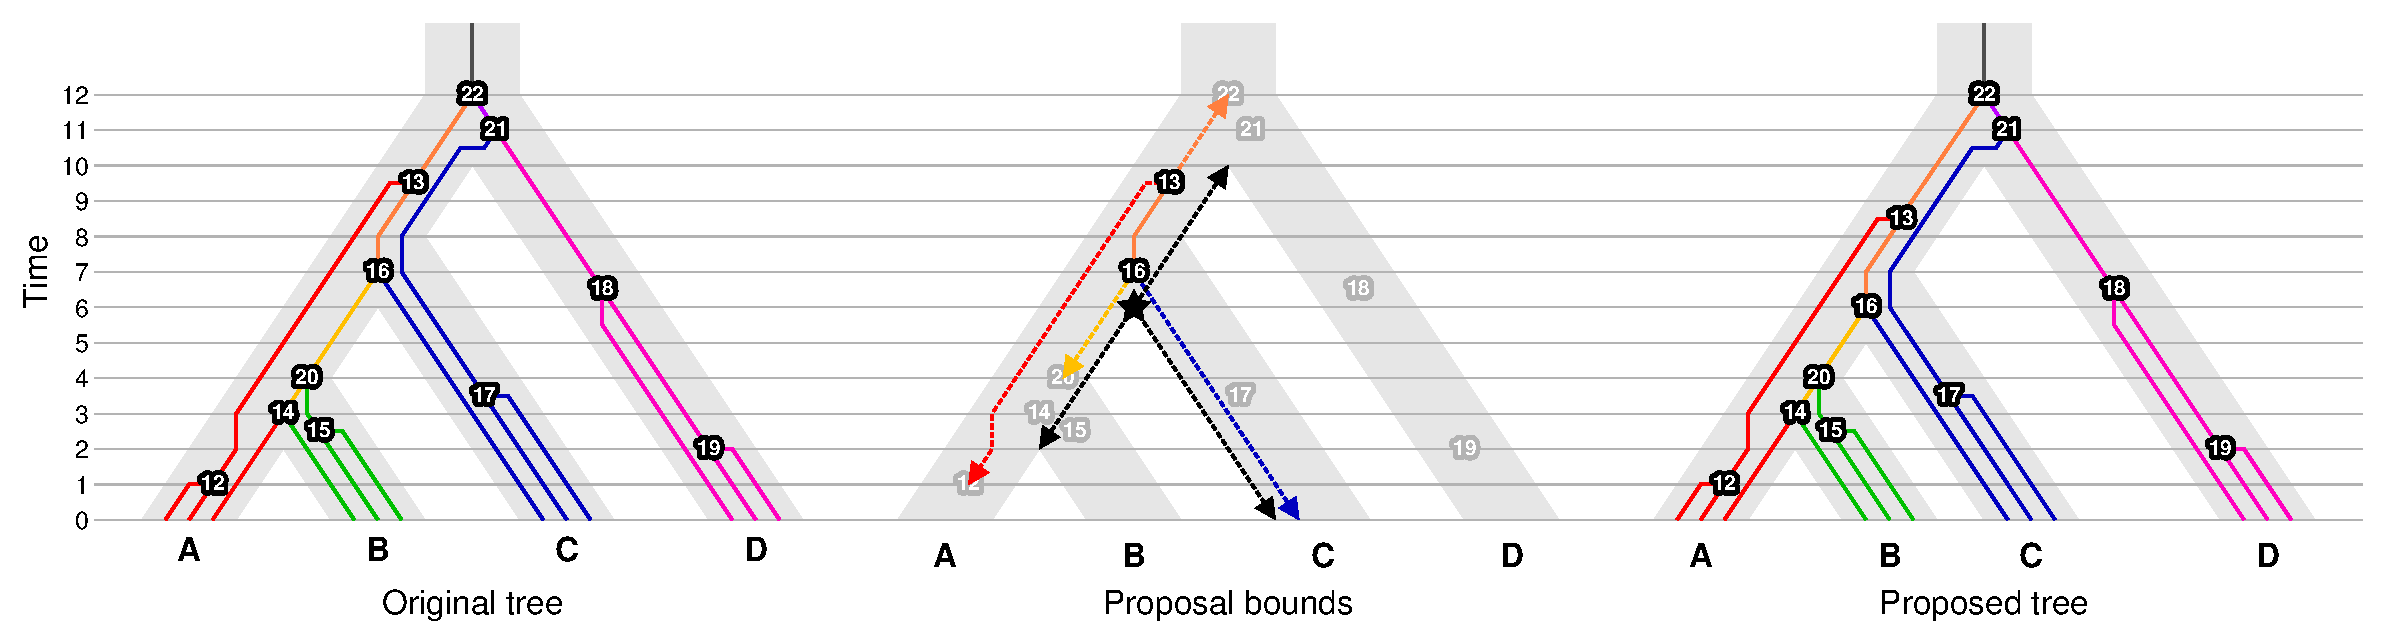
\includegraphics[width=\textwidth]{coordinated_uniform.pdf}
\caption
{Illustration of the CoordinatedUniform move. An example gene tree is embedded
within a four-taxon asymmetric species tree. Internal gene tree nodes
are numbered, species leaves lettered. The ABC node is represented by a star
in the middle step. Dashed lines are connected component and ABC
node child and parent branches.}
\label{fig:coordinatedUniform}
\end{figure}

The step after selecting a species tree node is to determine which internal
gene tree nodes will also be moved. CoordinatedUniform moves every gene tree
node $s$ in every gene tree which meets all of the following requirements:

\begin{enumerate}
\item at least one descendant individual of $s$ is also a
descendant individual of the \textit{left} child of $S$
\item at least one descendant individual of $s$ is also a
descendant individual of the \textit{right} child of $S$
\item all descendent individuals of $s$ are also
descendent individuals of $S$
\end{enumerate}

Descendent individuals of a gene tree node $s$ are gene tree leaf nodes which
have $s$ as an ancestor. Descendent individuals of a species tree node $S$ are
gene tree leaf nodes belonging to any extant species which has $S$ as an
ancestor. In the example, the left child of $S$ is the AB node, and the right
child of $S$ is the C node. The following internal nodes in the gene tree meet
requirement (1) 12, 13, 14, 15, 16, 20, 22; requirement (2) 13, 16, 17, 21,
22; and requirement (3) 12, 13, 14, 15, 16, 17, 20.

The only nodes in the example meeting all three requirements are 13 and 16.
These nodes are connected by a gene tree branch, making them a single
connected component. The connected component has three child branches (dashed
red, yellow and blue lines) and one parent branch (dashed orange line).

To determine the lower bound for the move, we must first identify the shortest
branch out of all connected component child branches and species tree node $S$
child branches. In the example the connected component child branches have
lengths of 3, 7 and 8.5, and the species tree node child branches have lengths 4
and 6 (Figure~\ref{fig:coordinatedUniform}). The lower bound is therefore the
original species tree node height $t(S) - 3 = 6 - 3 = 3$.

To determine the upper bound we use the shortest branch out of all connected
component parent branches and the species tree node $S$ parent branch. The
parent branch of the single connected component has a length of 2.5, and
the parent branch of $S$ has a length of 4. The upper bound is therefore
$t(S) + 2.5 = 6 + 2.5 = 8.5$.

A new species tree node height $t'(S)$ between 3 and 8.5 is chosen uniformly
at random. Within this range, if the connected component node heights are
changed by $\eta = t'(S) - t(S)$, no topology changes are induced or required.
In our example the new height is 5, so $\eta = 5 - 6.5 = -1.5$. After the
height of the species tree node $S$ and all connected component gene tree
nodes are changed by $\eta = -1.5$ the proposal is complete
(Figure~\ref{fig:coordinatedUniform}).

\end{document}
